\chapter{Problem Approach and Results} % (fold)
\label{cha:problem_approach_and_results}
\headermark{Problem Approach and Results}

Envisioning a system-wide performance optimization of a Ruby on Rails application requires targeting all the components involved from the previously mentioned centric perspective---Ruby on Rails. Conducting benchmarks, tweaking configurations, developing improved solutions and evaluating the results must be accomplished with this philosophy in mind. 

It is also necessary to perform these activities using a fair base of comparison. The most important rules used when benchmarking were:
\begin{description}
  \item[Same tests:] Use the same tests when testing component alternatives and, when impossible, keep their disparities to a minimum;
  \item[Same hardware:] Use the same hardware when testing a given component;
  \item[Similar configurations:] Use equal or, at the very least, similar configurations for all the components involved. Exceptions can be made when the purpose of the test is to benchmark the behavior with the default configurations.
\end{description}

Two distinct machines were used during this research. Due to hardware malfunction, the initial computer had to be replaced with a different one. ``Machine 1'' one was used on all the OS-related work, while ``Machine 2'' was used for all the activities related to the remaining components. Their specifications are listed on table~\ref{tab:machines_hardware_specification}.
\begin{table}[ht]
  \centering
  \caption{Hardware Specifications of the Machines in Use}
  \label{tab:machines_hardware_specification}
  
  \begin{tabular}{p{0.085\textwidth}|p{0.42\textwidth}|p{0.42\textwidth}}
    & \multicolumn{1}{c|}{\textbf{\textsc{Machine 1}}} & \multicolumn{1}{c}{\textbf{\textsc{Machine 2}}} \\ \hline

    \textbf{\textsc{CPU}} & Intel Core 2 Quad Q9300 @ 2.50GHz (FSB @ 1333MHz) & Intel Core 2 Duo ~\,E8400 @ 3.0GHz (FSB @ 1333MHz) \\ \hline
    \textbf{\textsc{RAM}} & 2x2GB DDR2 (800 MHz, Dual Channel) & 4x2GB DDR2 (800 MHz, Dual Channel) \\ \hline
    \textbf{\textsc{Hard Drive}} & Seagate ST3500620AS 500GB SATA, 16MB Cache & Seagate ST3750630AS 750GB SATA, 16MB Cache \\
  
  \end{tabular}
\end{table}

When benchmarking, the same software versions were used across all systems and environments. Table~\ref{tab:software_versions} explicits the software versions that were used.
\begin{table}[ht]
  \centering
  \caption{Software Versions in Use}
  \label{tab:software_versions}
  
  \begin{tabular}{p{0.25\textwidth}|p{0.25\textwidth}}
    \multicolumn{1}{c|}{\textbf{\textsc{Software/Package}}} & \multicolumn{1}{c}{\textbf{\textsc{Version}}} \\ \hline
    
    MRI & 1.8.7 (patchlevel 249) \\ \hline
    YARV & 1.9.1 (patchlevel 378) \\ \hline
    Rails & 2.3.5 \\ \hline
    FreeBSD & 8 \\ \hline
    Linux Kernel & 2.6.26 \\ \hline
    hdparm & 9.15 \\ \hline
    gzip & 1.3.12 \\ \hline
    lame & 3.98.2 \\ \hline
    vorbis-tools & 1.2.0 \\ \hline
    Apache & 2.2.14 \\ \hline
    Nginx & 0.7.64 \\ \hline
    Cherokee & 0.99.42 \\ \hline
    Thin & 1.2.7 \\ \hline
    Unicorn & 0.97.0 \\ \hline
    Passenger & 2.2.11 \\ \hline
    autobench & 2.1.2 \\ \hline
    httperf & 0.9.0 \\ \hline
    GCC & 4.3.4 \\
        
  \end{tabular}
\end{table}
All packages were compiled from source using GCC with \textit{``-O2 -march=nocona -pipe''} as their compilation flags.

To achieve the objectives established in chapter~\ref{cha:problem_statement}, some activities were performed.

First of all, to create the centralized set of conventions and guidelines for scaling Ruby on Rails applications, there is need to analyze and benchmark all worthy alternatives for each component.

In order to facilitate the process of profiling Rails applications by building new and intuitive tools while updating the existing ones, Rails and Ruby must be improved and tweaked to accommodate each other's changes.

Finally, to improve the global awareness on this issue's importance there is need to gather the benefits associated with it, provide a smoother transition by updating famous Rails plugins, increase this subjects' notoriety by updating one of the most renowned Ruby on Rails projects---Redmine---and by publishing a series of articles about performance optimization on the \textit{Rails Magazine} and, ultimately, initiate a performance-oriented continuous integration for Rails by developing a benchmarking suite aimed at the framework itself.

In order to accomplish the aforementioned tasks, every component was specifically addressed. The work done is presented and explained in the following sections.

\section{Operating Systems} % (fold)
\label{solution:sec:operating_systems}

Using Linux and BSD, the focus on this system component was to create generic benchmarking tools, determine the operating system in which common web servers perform better and to determine the OS in which the official Ruby interpreters have the best performance.

As exposed in chapter~\ref{state:sec:operating_systems}, Windows is not a suitable OS for production environments of Ruby on Rails applications because of its poor and inefficient support for this applications that use this framework, being excluded from further research. On the other hand, Mac OS X Server requires specific hardware so any comparison's would not be rigorous. Its performance is expected to be similar to BSD systems since, as mentioned in section~\ref{tech:sec:operating_systems}, its kernel is based on this OS, reducing the downside of its exclusion.

\begin{comment}
Create generic and specific tools of OS performance measurement

Find the best OS for Rails by benchmarking the most likely candidates (same hardware)

Tweak OSes configurations

OSes are already highly optimized, OS development doesn't make much sense
\end{comment}


\subsection{Development}
Concerning development, a generic benchmarking script was created. This script was based on a few commonly found tools on Unix setups and consists on 5 micro-tests and 1 macro-test, respectively:
\begin{enumerate}
  \item Use hdparm to time cached reads on the disk;
  \item Compress a 2.5GB file to ZIP format using gzip;
  \item Uncompress the previously created archive;
  \item Convert a 214MB WAV file to MP3 using lame;
  \item Convert the same 214MB WAV file to OGG using vorbis-tools;
  \item Parallelly run all the aforementioned benchmarks while extracting, compiling, installing and removing PHP 5.2.12.
\end{enumerate}
The script measures the real amount of time needed to accomplish each task, the number of voluntary context switches and the average CPU usage. GNU time is used to make all measurements except in the first test, since hdparm itself measures the amount of cached data read in 2 seconds yielding results in MB/second. All tests are ran a configurable amount of times to cancel circumstantial issues, the default being 3. Exception is made on the last test which is very heavy and lengthy, so it only runs once.

The first test aims at testing hard drive access speed, which are dependent on the filesystem in use and the OS's IO management. The second and third tests are more complex since but similar. Both read a file with considerable size from the disk, convert it and write the result. However, the main bottleneck happens when writing the result file since writing is slower process than reading and the ZIP algorithm is lightweight and fast. The fourth and fifth tests are more CPU-intensive. Audio format conversions tend to demand a significant amount of processing power. The tools in use---lame and vorbis-tools---stress the OS even further by using multiple processes and threads, inducing various context switches. Finally, the last test aims at testing the OS's ability to manage a high workload since multiple heavy tasks are being carried simultaneously, involving concurrent IO, context switches, scheduling and a few other core tasks.

\subsection{Benchmarking}
The benchmarking phase had the clear goal of defining which is the likely best OS to invest in the remaining work. It was also very important to gather data about each OS/distribution behavior so that it would be inserted in the aforementioned guidelines in conventions.

\subsubsection{Generic Benchmarking of Linux distributions}
First of all, it was important to choose one of the Linux distributions mentioned in section~\ref{tech:sec:operating_systems} to be stacked against FreeBSD, the most popular BSD distribution. A benchmark using the aforementioned generic script was performed on Ubuntu Server, Debian, CentOS and Gentoo. All distributions were running their default configurations for all packages. The results are shown in table~\ref{TABELA TABELA}.
\\
TABELA TABELA
\\
Gentoo's performance is better by a slight margin in the first test, yielding results which range from 3\% to 7\% better than the other distributions. The second test yielded similar results, with Debian's performance being very close to Gentoo's. CentOS shows serious issues in this test, being 502\% slower than Gentoo. Regarding the third test, Gentoo showed the best result, followed by Debian's. CentOS yields very poor results again, being 1903\% slower than Gentoo. Quite unexpectedly, CentOS had the best performance in the fourth test by a comfortable margin, with Debian's results being the second best once again. Ubuntu yielded the best performance in the fifth test, with Debian and Gentoo having very close results. CentOS shows the worst results by a considerable 13\% margin. Finally, Debian yielded the best results in the final test by a substantial margin. CentOS's results, once more, show a considerable performance deficiency when compared to the other distributions' results.

According to these results, Gentoo is the best distribution in CPU usage and IO operations on a single instance, present in tests 1, 2 and 3. When it comes to almost pure CPU usage, CentOS and Ubuntu yield the best results. Last but not least, Debian showed an impressive behavior handling concurrent tasks present in the last test.

CentOS's behavior was unstable and inconsistent. Given these results, it was discarded from future work.

\subsubsection{Web Server Benchmarking on Linux distributions}
Since there are still 3 possible Linux distributions to be compared with FreeBSD, a different benchmark was endured. This time, its focus was oriented towards web server performance.

This test used a simple static HTML page served by either Apache or Nginx. Using Ubuntu Server, Debian and Gentoo many requests/concurrency combinations were used, namely:
\begin{enumerate}
  \item 10000 requests, 1000 concurrent;
  \item 100000 requests, 1000 concurrent;
  \item 100000 requests, 10000 concurrent.
\end{enumerate}
Apache's ab utility was used to perform the tests. All of them were local, providing zero network overhead since the goal is to measure raw web server performance on each OS. If any request took more than 30 seconds to be replied to the test was considered a failure, as a higher response time is not acceptable in real world applications. The web server configurations were not the default ones on this test. Since some distributions loaded more modules than others and this could have a significant impact the web server performance, all unnecessary modules and options for this benchmark were removed from the configurations.

Regarding the Apache benchmark, table~\ref{WWWWWWWWWWWW} shows that Gentoo had the best performance in the first Apache test, with Debian achieving similar results. Ubuntu, however, did not cope with the other's behavior, needing a considerable amount of extra time to accomplish the same test. As seen on table~\ref{WWWWWWWWWWWWW}, Gentoo showed the best performance in the second Apache test. Debian had a considerably worse performance and Ubuntu failed this test as many requests took more than the aforementioned 30 seconds to be replied to. Finally, table~\ref{WWWWWWWWWWWWWWWW} shows the results of the last Apache benchmark, where all distributions failed to successfully complete the benchmark except Gentoo, which needed a high average amount of time to complete but was still able to reply to all requests within the established time limit.

Concerning the Nginx benchmark, table~\ref{WWWWWWWWWWWW} shows that this time it was Debian to achieve the best result on the first benchmark, yielding impressive performance. The results of the second test are shown on table~\ref{WWWWWWWWWWWW} and Debian seems to be the best performing distribution once again. The third test's results showed some unexpected results since, similarly to the Apache benchmark, neither Debian nor Ubuntu were able to cope with the high demand, leaving the best result to Gentoo which was the only distribution to successfully complete the final test. These results can be found in table~\ref{WWWWWWWWWWWW}.

Gentoo showed an excellent behavior when scaling. The difference in average time taken for each request on tests 1 and 2 of both web servers is remarkably small. It was also the only distribution to be able to cope with 100000 requests with 10000 of them concurrent, either on Apache and Nginx. These results allowed to confidently decide that Gentoo is the best distribution to compare to FreeBSD.

\subsubsection{Ruby Benchmark on Gentoo Linux and FreeBSD}
Given this research's scope, it is important to determine which of the aforementioned OSes---Gentoo Linux or FreeBSD---provide the best environment for a Ruby on Rails application. A Ruby on Rails application, as the name implies, is written in Ruby just like the framework it is using. Therefore, Ruby is a core component from Rails' perspective. The official Ruby interpreters are likely to yield different performance results on different OSes since they are mainly developed in Linux and then ported to other Operating Systems. If we take into account the already known differences stated on section~\ref{state:sec:operating_systems}, benchmarking this core component is likely to yield different results and to enable a confident assertion about the OS in which it is developed---Linux---is the best for a Ruby on Rails application or not.

For this benchmark, Antonio Cangiano's Ruby benchmarking suite~\cite[ruby-benchmarking-suite] was used. It currently contains 62 micro benchmarks which test specific Ruby features, 8 macro benchmarks which test multiple Ruby features in a single test and 3 RDoc-related benchmarks. Each benchmark ran 5 times and had a 300 second timeout. This high test variety provides a wide coverage of many Ruby features, solidly asserting about the interpreter's overall performance. All tests were ran using both Ruby interpreters, MRI (Ruby 1.8) and YARV (Ruby 1.9), in both operating systems.
\\
TABELA TABELA
\\
As seen on table~\ref{TABELA MRI}, MRI has a better overall performance in Linux. The average improvement is of 29.34\%.

Table~\ref{TABELA YARV} shows the results of the YARV benchmark. Similarly to MRI's benchmark, YARV has a better overall performance in Linux. The average improvement is 22.21\% on this test.

After eliminating FreeBSD from the benchmarking subjects, Gentoo Linux is the OS that will be used in future work. It is very stable, configurable and enables improved performance of Ruby-related software when compared to FreeBSD.

\begin{comment}
Use the generic benchmarks mentioned above

Web server benchmark (Nginx/Apache on each disto)

Ruby benchmarks on each OS

Show results and analysis
\end{comment}


\subsection{Tweaking}
There are many configurations and options that can be fine-tuned on an Operating System. Sysctl enables kernel parameter configuration at runtime. The aforeshown web server benchmarks required some optimization changes to improve the system's stability under high-load. These are shown on table~\ref{tab:sysctl}.
\begin{table}[ht]
  \centering
  
  \begin{tabular}{p{0.05\textwidth}|p{0.32\textwidth}|p{0.25\textwidth}}
    \textsc{\#} 
  & \textsc{Name}
  & \textsc{Value} \\
  \hline
  1 & net.core.rmem\_max & 16777216 \\
  2 & net.core.wmem\_max & 16777216 \\
  3 & net.ipv4.tcp\_rmem & 4096~\, 87380~\, 16777216 \\  
  4 & net.ipv4.tcp\_wmem & 4096~\, 87380~\, 16777216 \\
  5 & net.core.netdev\_max\_backlog & 4096 \\
  6 & net.core.somaxconn & 4096 \\
  7 & net.ipv4.tcp\_tw\_reuse & 1 \\
  8 & net.ipv4.tcp\_tw\_recycle & 1 \\
  9 & net.ipv4.tcp\_fin\_timeout & 15 \\
  10 & net.ipv4.tcp\_timestamps & 0 \\
  11 & net.ipv4.tcp\_orphan\_retries & 1 \\
  
  \end{tabular}
  \caption{Sysctl options and values}
  \label{tab:sysctl}
\end{table}
Options 1, 2, 3 and 4 increase the TCP buffers on read/write, improving the system performance when dealing with big transfers. Options 5 and 6 increase the number of connections which are allowed to be queued behind a busy kernel. Options 7 and 8 enable socket reusing and fast socket recycling. Option 9 decreases the time allowed for a socket to exists without a connection. Option 10 disables timestamps in packet headers, reducing the packet's size. Finally, option 11 decreases the number of retries before killing the TCP connection.

The number of opened files limit also had to be increased in the system's limits configuration. It defaults to 1024 which is very low on a server, taking into account that each socket connection uses a file on a UNIX system. This would generally cap the system's concurrency ability to ~1000, so it was increased to 65536.

A few other options are worth investigating. Many server-oriented distributions use the Deadline IO scheduler which gives a higher priority to read requests, while others use the CFQ scheduler which is commonly found on desktop systems. Preemption should also be disabled on a server kernel. In non-preemptive configurations, kernel code runs until completion---the scheduler can't touch it until it's finished. Server kernels should also have their timer interrupt rate set to 100Hz, which causes higher latency but lower overhead, yielding superior raw processing power.

On a side note, all the aforementioned configuration changes were in use in all benchmarks.

\section{Ruby} % (fold)
\label{solution:sec:ruby}
Concerning this component, the main focus was divided into four core activities. First of all, determining the real benefits of upgrading to the latest Ruby 1.9. After that, focus would shift towards porting \textit{Escolinhas.pt} to Ruby 1.9. Then, the aim was to improve YARV's GC by increasing its flexibility. Finally, Ruby's profiling and information retrieval capabilities were enhanced.

There are many interpreters being used in production environments whose characteristics were explored in Section~\ref{tech:sec:ruby}. Unfortunately, none except YARV fully support the most recent specification---1.9. It is likely that focusing on soon to be outdated solutions is not worthy. For this reason, YARV was the interpreter targeted for improvements.

Determining the performance benefits from upgrading to the most recent version of Ruby, analyzing the effort needed to accomplish it, improving one of YARV's main bottlenecks related with Rails---the garbage collector---and greatly enhancing its profiling capabilities were the general goals of the work presented in this section.

\subsection{Benchmarking}
As mentioned in Section~\ref{state:sec:ruby} the new Ruby interpreter, YARV, is supposed to significantly improve performance over its predecessor, MRI. Its first release happened more than two years ago and its adoption is still very low, despite having new features and supposedly better performance. Porting existing applications requires some development effort as there are small changes on existing functionality and behavior. Having said that Rails can easily have scalability issues, it would be expected that this version's adoption would rise considerably fast but, however, this is not currently happening.

To increase the community's awareness of the benefits of upgrading, these need to be accurately determined. The Ruby benchmark mentioned and explained on Section~\ref{solution:sec:operating_systems} was rerun to exhibit the interpreter's disparity when it comes to performance, as shown on table~\ref{tab:mri_yarv_benchmark}.

\begin{center}
\renewcommand{\arraystretch}{0.85}
\normalsize
  \begin{longtable}{l|c|c|c|c}
  \caption[MRI and YARV Benchmark Comparison]{MRI and YARV Benchmark Comparison} \label{tab:mri_yarv_benchmark} \\

  \multicolumn{1}{c|}{\textbf{Benchmark}} & \textbf{Input Size} & \textbf{MRI (1.8.7)} & \textbf{YARV (1.9.1)} & \textbf{Ratio} \\ \hline 
  \endfirsthead

  \multicolumn{5}{c}%
  {{\bfseries \tablename\ \thetable{} --- continued from previous page}} \\
  \multicolumn{1}{c|}{\textbf{Benchmark}} & \textbf{Input Size} & \textbf{MRI (1.8.7)} & \textbf{YARV (1.9.1)} & \textbf{Ratio} \\ 
  \endhead

  \multicolumn{5}{r}{{\tablename\ \thetable{} --- continued on the next page}} \\ \hline
  \endfoot

  \endlastfoot

  macro/cal & 500 & 1.990 & \textbf{0.289} & 589.28\% \\ \hline
  macro/dirp & 10000 & \textbf{0.386} & 0.393 & 2.04\% \\ \hline
  macro/gzip & 100 & 6.141 & \textbf{5.979} & 2.70\% \\ \hline
  macro/hilbert\_matrix & 10 & 0.036 & \textbf{0.002} & 1509.42\% \\ \hline
  macro/hilbert\_matrix & 20 & 0.335 & \textbf{0.031} & 984.21\% \\ \hline
  macro/hilbert\_matrix & 30 & 1.367 & \textbf{0.154} & 789.44\% \\ \hline
  macro/hilbert\_matrix & 40 & 3.866 & \textbf{0.477} & 710.68\% \\ \hline
  macro/hilbert\_matrix & 50 & 8.868 & \textbf{1.256} & 605.76\% \\ \hline
  macro/hilbert\_matrix & 60 & 18.399 & \textbf{3.024} & 508.39\% \\ \hline
  macro/list & 1000 & 0.053 & \textbf{0.026} & 102.35\% \\ \hline
  macro/list & 10000 & 7.154 & \textbf{2.758} & 159.43\% \\ \hline
  macro/mpart & 300 & 0.039 & \textbf{0.034} & 16.56\% \\ \hline
  macro/norvig\_spelling & 50 & 8.562 & ArgumentError &  \\ \hline
  macro/observ & 100000 & 0.612 & \textbf{0.360} & 69.88\% \\ \hline
  macro/parse\_log & 100 & 1.151 & \textbf{0.309} & 271.94\% \\ \hline
  macro/pi & 1000 & 0.026 & \textbf{0.024} & 7.46\% \\ \hline
  macro/pi & 10000 & 2.127 & \textbf{2.034} & 4.61\% \\ \hline
  macro/rcs & 100 & 0.753 & \textbf{0.581} & 29.70\% \\ \hline
  macro/sudoku & 1 & 10.153 & \textbf{1.661} & 511.27\% \\ \hline
  micro/app\_factorial & 5000 & StackError & 0.037 &  \\ \hline
  micro/app\_fib & 30 & 1.587 & \textbf{0.189} & 741.29\% \\ \hline
  micro/app\_fib & 35 & 17.854 & \textbf{2.099} & 750.68\% \\ \hline
  micro/app\_mandelbrot & 1 & 1.899 & \textbf{0.277} & 585.27\% \\ \hline
  micro/app\_pentomino & 1 & SignalException & 24.784 &  \\ \hline
  micro/app\_tak & 7 & 1.173 & \textbf{0.143} & 719.77\% \\ \hline
  micro/app\_tak & 8 & 3.405 & \textbf{0.414} & 722.62\% \\ \hline
  micro/app\_tak & 9 & 8.910 & \textbf{1.091} & 716.51\% \\ \hline
  micro/app\_tarai & 3 & 3.873 & \textbf{0.492} & 686.81\% \\ \hline
  micro/app\_tarai & 4 & 4.670 & \textbf{0.604} & 673.22\% \\ \hline
  micro/app\_tarai & 5 & 5.654 & \textbf{0.731} & 672.95\% \\ \hline
  micro/binary\_trees & 1 & 54.757 & \textbf{12.500} & 338.06\% \\ \hline
  micro/count\_multithreaded & 1 & \textbf{0.004} & 0.006 & 40.88\% \\ \hline
  micro/count\_multithreaded & 2 & \textbf{0.009} & 0.012 & 41.65\% \\ \hline
  micro/count\_multithreaded & 4 & \textbf{0.017} & 0.025 & 45.27\% \\ \hline
  micro/count\_multithreaded & 8 & \textbf{0.034} & 0.049 & 46.36\% \\ \hline
  micro/count\_multithreaded & 16 & \textbf{0.067} & 0.100 & 48.25\% \\ \hline
  micro/count\_shared\_thread & 1 & \textbf{0.044} & 0.061 & 39.60\% \\ \hline
  micro/count\_shared\_thread & 2 & \textbf{0.044} & 0.061 & 39.45\% \\ \hline
  micro/count\_shared\_thread & 4 & \textbf{0.044} & 0.061 & 38.36\% \\ \hline
  micro/count\_shared\_thread & 8 & \textbf{0.044} & 0.062 & 40.22\% \\ \hline
  micro/count\_shared\_thread & 16 & \textbf{0.045} & 0.062 & 38.67\% \\ \hline
  micro/eval & 1000000 & \textbf{1.843} & 5.892 & 219.67\% \\ \hline
  micro/fannkuch & 6 & 0.005 & \textbf{0.003} & 54.48\% \\ \hline
  micro/fannkuch & 8 & 0.398 & \textbf{0.252} & 57.81\% \\ \hline
  micro/fannkuch & 10 & 44.995 & \textbf{29.300} & 53.57\% \\ \hline
  micro/fasta & 1000000 & 37.028 & \textbf{13.992} & 164.65\% \\ \hline
  micro/fiber\_ring & 10 & LoadError & 0.000 &  \\ \hline
  micro/fiber\_ring & 100 & LoadError & 0.018 &  \\ \hline
  micro/fiber\_ring & 1000 & LoadError & 1.724 &  \\ \hline
  micro/fractal & 5 & 4.520 & \textbf{3.004} & 50.48\% \\ \hline
  micro/gc\_array & 1 & 44.990 & \textbf{39.619} & 13.56\% \\ \hline
  micro/gc\_mb & 500000 & 0.687 & \textbf{0.173} & 297.95\% \\ \hline
  micro/gc\_mb & 1000000 & 1.513 & \textbf{0.346} & 337.27\% \\ \hline
  micro/gc\_mb & 3000000 & 3.535 & \textbf{1.087} & 225.32\% \\ \hline
  micro/gc\_string & 1 & 7.874 & \textbf{3.090} & 154.80\% \\ \hline
  micro/knucleotide & 1 & 1.396 & \textbf{0.826} & 68.93\% \\ \hline
  micro/lucas\_lehmer & 9689 & \textbf{4.019} & 4.611 & 14.73\% \\ \hline
  micro/lucas\_lehmer & 9941 & \textbf{4.342} & 4.980 & 14.68\% \\ \hline
  micro/lucas\_lehmer & 11213 & \textbf{6.174} & 7.096 & 14.93\% \\ \hline
  micro/lucas\_lehmer & 19937 & \textbf{33.143} & 38.069 & 14.87\% \\ \hline
  micro/mandelbrot & 1 & 55.460 & \textbf{30.207} & 83.60\% \\ \hline
  micro/mbari\_bogus1 & 1 & StackError & 0.008 &  \\ \hline
  micro/mergesort & 1 & 1.914 & \textbf{0.659} & 190.40\% \\ \hline
  micro/mergesort\_hongli & 3000 & 4.423 & \textbf{1.108} & 299.34\% \\ \hline
  micro/meteor\_contest & 1 & 25.352 & \textbf{7.633} & 232.14\% \\ \hline
  micro/monte\_carlo\_pi & 10000000 & 12.178 & \textbf{7.828} & 55.58\% \\ \hline
  micro/nbody & 100000 & 7.046 & \textbf{5.569} & 26.53\% \\ \hline
  micro/nsieve & 9 & 15.221 & NoMethodError &  \\ \hline
  micro/nsieve\_bits & 8 & 19.753 & \textbf{2.385} & 728.28\% \\ \hline
  micro/open\_many\_files & 50000 & \textbf{0.211} & 0.245 & 16.05\% \\ \hline
  micro/partial\_sums & 2500000 & 18.003 & \textbf{14.396} & 25.05\% \\ \hline
  micro/primes & 3000 & 5.057 & \textbf{0.012} & 43396.39\% \\ \hline
  micro/primes & 30000 & SignalException & 0.128 &  \\ \hline
  micro/primes & 300000 & SignalException & 1.404 &  \\ \hline
  micro/primes & 3000000 & SignalException & 17.761 &  \\ \hline
  micro/quicksort & 1 & 7.116 & \textbf{1.432} & 396.99\% \\ \hline
  micro/read\_large & 100 & 6.337 & \textbf{2.441} & 159.65\% \\ \hline
  micro/regex\_dna & 20 & \textbf{2.644} & 2.797 & 5.78\% \\ \hline
  micro/reverse\_compliment & 1 & 3.702 & \textbf{2.782} & 33.08\% \\ \hline
  micro/simple\_connect & 1 & \textbf{0.134} & 0.216 & 60.82\% \\ \hline
  micro/simple\_connect & 100 & \textbf{0.143} & 0.143 & 0.40\% \\ \hline
  micro/simple\_connect & 500 & 0.175 & \textbf{0.173} & 0.72\% \\ \hline
  micro/simple\_server & 1 & \textbf{0.134} & 0.138 & 3.02\% \\ \hline
  micro/simple\_server & 100 & \textbf{0.136} & 0.138 & 1.89\% \\ \hline
  micro/simple\_server & 100000 & 1.427 & \textbf{1.411} & 1.12\% \\ \hline
  micro/so\_ackermann & 7 & 0.494 & \textbf{0.059} & 734.56\% \\ \hline
  micro/so\_ackermann & 9 & StackError & 0.957 &  \\ \hline
  micro/so\_array & 9000 & 6.867 & \textbf{1.938} & 254.26\% \\ \hline
  micro/so\_count\_words & 100 & \textbf{2.408} & 2.831 & 17.52\% \\ \hline
  micro/so\_exception & 500000 & \textbf{8.009} & 8.324 & 3.93\% \\ \hline
  micro/so\_lists & 1000 & 8.649 & \textbf{4.483} & 92.91\% \\ \hline
  micro/so\_lists\_small & 1000 & 1.741 & \textbf{0.905} & 92.30\% \\ \hline
  micro/so\_matrix & 60 & 1.924 & \textbf{0.592} & 224.80\% \\ \hline
  micro/so\_object & 500000 & 1.424 & \textbf{0.413} & 244.44\% \\ \hline
  micro/so\_object & 1000000 & 2.825 & \textbf{0.817} & 245.87\% \\ \hline
  micro/so\_object & 1500000 & 4.265 & \textbf{1.224} & 248.29\% \\ \hline
  micro/so\_sieve & 4000 & 54.784 & \textbf{8.650} & 533.31\% \\ \hline
  micro/socket\_transfer\_1mb & 10000 & 0.353 & \textbf{0.306} & 15.40\% \\ \hline
  micro/socket\_transfer\_1mb & 1000000 & 0.356 & \textbf{0.304} & 17.28\% \\ \hline
  micro/spectral\_norm & 100 & 0.932 & \textbf{0.233} & 300.57\% \\ \hline
  micro/string\_concat & 10000000 & 5.655 & \textbf{1.525} & 270.78\% \\ \hline
  micro/sum\_file & 100 & 9.920 & \textbf{3.817} & 159.90\% \\ \hline
  micro/word\_anagrams & 1 & 7.750 & \textbf{3.775} & 105.31\% \\ \hline
  micro/write\_large & 100 & 0.157 & \textbf{0.147} & 6.51\% \\ \hline
  rdoc/against\_itself\_darkfish & 1 & 13.118 & \textbf{6.991} & 87.65\% \\ \hline
  rdoc/against\_itself\_ri & 1 & 12.854 & \textbf{5.580} & 130.35\% \\ \hline
  \textbf{Total} & \multicolumn{1}{l|}{\textbf{}} & \textbf{679.880} & \textbf{325.398} & \textbf{108.94\%} \\
  \end{longtable}
\end{center}

As expected, YARV shows excellent results on this benchmark, in comparison with MRI. It is approximately 109\% faster than the older 1.8 interpreter. Concerning memory usage, MRI used an average 46,34MB of memory during the whole benchmark while YARV only consumed 30,81MB. Regarding specific tests, YARV is generally faster by there is a notable exception: threads. As explained in Section~\ref{tech:sec:ruby}, MRI uses green threads while YARV supports native threads. Green threads emulate multithreaded environments but there is no parallel computing at all since they do not use multiple processing units. They have, however, a significantly low spawning overhead, contrary to native threads. The previously shown threading tests, where MRI yielded better results than YARV, are very fast. For this reason, the overhead of spawning native threads for such a small test duration had a considerable impact in the overall performance of YARV, resulting in poorer performance. Heavier tests would likely yield different results, given that native threads are actually capable of running on different processing units.

Notwithstanding this exception, YARV shows significant performance improvements overall and this fact is likely to motivate developers to switch to this version.

It is also critical to determine the performance differences on a real Rails application. As this is also related to the web server in use, this subject will be researched throughly on Section~\ref{solution:sec:rails_web_servers}.

\subsection{Development}
The development phase involved many distinct activities. The details on each one of them are explored and explained below.

\subsubsection{Porting Escolinhas.pt to Ruby 1.9}
\textit{Escolinhas.pt} has over 70 models and database tables, over 130000 lines of Ruby code, uses over 40 Rails plugins and gems, and there are currently more than 10 development branches. It is a heavy and complex full-featured application, making it a great subject to evaluate the effort needed to port an application to Ruby 1.9.

This process was fairly simple. The main issue was related to character encodings in Portuguese literal strings on the source code and database, which emerged from the heavy changes regarding encoding handling in Ruby 1.9. A patch to fix literal string encoding can be found on appendix~\ref{ap:ruby19_encoding_patch}. Ruby 1.9 also requires developers to set the default encoding for each file inside a comment in the beginning, or else it will use the default ASCII-8BIT which has its known limitations. A task was developed to manage the default encoding in all files of a Ruby project and is presented on appendix~\ref{ap:ruby19_encoding_task}.

Other issues were mainly related to extracted functionality and syntax changes. The most common ones were:
\begin{itemize}
  \item \textit{Object.type} changed to \textit{Object.class.name};
  \item The \textit{String} class no longer has the \textit{normalize} method;
  \item The case statement no longer supports ``:'' to separate the match word from the action to be taken.
\end{itemize}

As mentioned before, porting \textit{Escolinhas.pt} to Ruby 1.9 was a very fast and simple process. Measuring the effort in time units, porting to 1.9 accounted for less then 0.1\% of all the development endeavor. All changes were simple and straightforward. Taking the aforementioned performance benefits into account, porting an application to Ruby 1.9 is likely to be very worthy on most projects.

On a related matter, a considerable amount of effort is being made by the Ruby on Rails development team to automatically manage the encoding of Ruby files in Rails 3. Given that Ruby's encoding changes accounted for most part of the effort needed to port \textit{Escolinhas.pt} to Ruby 1.9, porting an application under Rails 3 should generally be effortless, as this version natively handles most of Ruby's encoding-related quirks.

\subsubsection{Increasing YARV's GC Flexibility}
Ruby Enterprise Edition, as exposed in Section~\ref{tech:sec:ruby}, allows users to set some GC parameters, providing adaptive performance. As mentioned in Section~\ref{state:sec:ruby}, many platforms benefit from this flexibility by adapting many GC parameters to their applications. Adding this functionality to YARV was the goal, and it currently supports the following settings:
\begin{description}
  \item[RUBY\_HEAP\_MIN\_SLOTS,] the initial number of heap slots. It also represents the minimum number of slots at all times (default: 10000);
  \item[RUBY\_HEAP\_SLOTS\_INCREMENT,] the number of new slots to allocate when all initial slots are used (default: 10000);
  \item[RUBY\_HEAP\_SLOTS\_GROWTH\_FACTOR,] the multiplicator used next time Ruby needs new heap slots (default: 1.8, meaning it will allocate 18000 new slots if the default settings are in use);
  \item[RUBY\_GC\_MALLOC\_LIMIT,] the number of C data structures that can be allocated before triggering the garbage collector. This one is very important since the default value makes the GC run when there are still empty heap slots, mainly due to Rails frequently allocating and deallocating large amounts of data (default: 8000000);
  \item[RUBY\_HEAP\_FREE\_MIN,] the number of free slots that should be present after GC finishes running. In case there are fewer slots than those defined, it will allocate new ones according to value of \textit{RUBY\_HEAP\_SLOTS\_INCREMENT} and the value of the previously mentioned \textit{RUBY\_HEAP\_SLOTS\_GROWTH\_FACTOR} parameters (default: 4096).
\end{description}
The developer can configure these options in the system's environment and the Ruby interpreter will detect and apply them to its internal configuration.

Appendix~\ref{ap:ruby19_configuration} contains a sample script which launches Ruby with a user-defined configuration. The parameters indicate that Ruby should start with more initial slots, have a higher threshold for triggering the GC and have a less exponential memory growth---1,1---instead of using the default 1,8 coefficient.

A benchmark comparing these configurations with the default ones was conducted and is presented on table~\ref{tab:flexible_yarv_benchmark}.
\begin{center}
\renewcommand{\arraystretch}{0.85}
\normalsize
  \begin{longtable}{l|c|c|c|c}
  \caption[Flexible YARV Benchmark]{Flexible YARV Benchmark} \label{tab:flexible_yarv_benchmark} \\

  \multicolumn{1}{c|}{\textbf{Benchmark}} & \textbf{Input Size} & \textbf{YARV} & \textbf{YARV (tweaked)} & \textbf{Ratio} \\ \hline 
  \endfirsthead

  \multicolumn{5}{c}%
  {{\bfseries \tablename\ \thetable{} --- continued from previous page}} \\
  \multicolumn{1}{c|}{\textbf{Benchmark}} & \textbf{Input Size} & \textbf{1.9.1 (Gentoo)} & \textbf{1.9.1(FreeBSD)} & \textbf{Ratio} \\ 
  \endhead

  \multicolumn{5}{r}{{\tablename\ \thetable{} --- continued on the next page}} \\ \hline
  \endfoot

  \endlastfoot

  macro/cal & 500 & 0.289 & \textbf{0.253} & 14.03\% \\ \hline
  macro/dirp & 10000 & \textbf{0.393} & 0.454 & 15.38\% \\ \hline
  macro/gzip & 100 & \textbf{5.979} & 5.991 & 0.20\% \\ \hline
  macro/hilbert\_matrix & 10 & 0.002 & \textbf{0.002} & 12.81\% \\ \hline
  macro/hilbert\_matrix & 20 & 0.031 & \textbf{0.027} & 13.03\% \\ \hline
  macro/hilbert\_matrix & 30 & 0.154 & \textbf{0.133} & 15.65\% \\ \hline
  macro/hilbert\_matrix & 40 & 0.477 & \textbf{0.399} & 19.47\% \\ \hline
  macro/hilbert\_matrix & 50 & 1.256 & \textbf{1.022} & 22.95\% \\ \hline
  macro/hilbert\_matrix & 60 & 3.024 & \textbf{2.296} & 31.72\% \\ \hline
  macro/list & 1000 & 0.026 & \textbf{0.025} & 7.04\% \\ \hline
  macro/list & 10000 & 2.758 & \textbf{1.418} & 94.42\% \\ \hline
  macro/mpart & 300 & 0.034 & \textbf{0.032} & 4.63\% \\ \hline
  macro/norvig\_spelling & 50 & ArgumentError & 4.781 &  \\ \hline
  macro/observ & 100000 & 0.360 & \textbf{0.336} & 7.14\% \\ \hline
  macro/parse\_log & 100 & \textbf{0.309} & 0.460 & 48.72\% \\ \hline
  macro/pi & 1000 & 0.024 & \textbf{0.023} & 3.31\% \\ \hline
  macro/pi & 10000 & 2.034 & \textbf{1.979} & 2.77\% \\ \hline
  macro/rcs & 100 & 0.581 & \textbf{0.491} & 18.16\% \\ \hline
  macro/sudoku & 1 & 1.661 & \textbf{1.570} & 5.77\% \\ \hline
  micro/app\_factorial & 5000 & 0.037 & \textbf{0.036} & 3.83\% \\ \hline
  micro/app\_fib & 30 & 0.189 & \textbf{0.177} & 6.47\% \\ \hline
  micro/app\_fib & 35 & 2.099 & \textbf{1.954} & 7.43\% \\ \hline
  micro/app\_mandelbrot & 1 & 0.277 & \textbf{0.242} & 14.64\% \\ \hline
  micro/app\_pentomino & 1 & 24.784 & \textbf{23.880} & 3.79\% \\ \hline
  micro/app\_tak & 7 & 0.143 & \textbf{0.138} & 3.93\% \\ \hline
  micro/app\_tak & 8 & 0.414 & \textbf{0.395} & 4.72\% \\ \hline
  micro/app\_tak & 9 & 1.091 & \textbf{1.054} & 3.58\% \\ \hline
  micro/app\_tarai & 3 & 0.492 & \textbf{0.485} & 1.54\% \\ \hline
  micro/app\_tarai & 4 & 0.604 & \textbf{0.585} & 3.31\% \\ \hline
  micro/app\_tarai & 5 & 0.731 & \textbf{0.708} & 3.27\% \\ \hline
  micro/binary\_trees & 1 & 12.500 & \textbf{11.870} & 5.30\% \\ \hline
  micro/count\_multithreaded & 1 & 0.006 & \textbf{0.006} & 3.11\% \\ \hline
  micro/count\_multithreaded & 2 & 0.012 & \textbf{0.012} & 3.74\% \\ \hline
  micro/count\_multithreaded & 4 & 0.025 & \textbf{0.024} & 4.68\% \\ \hline
  micro/count\_multithreaded & 8 & 0.049 & \textbf{0.047} & 4.26\% \\ \hline
  micro/count\_multithreaded & 16 & 0.100 & \textbf{0.095} & 4.93\% \\ \hline
  micro/count\_shared\_thread & 1 & 0.061 & \textbf{0.059} & 3.22\% \\ \hline
  micro/count\_shared\_thread & 2 & 0.061 & \textbf{0.059} & 3.06\% \\ \hline
  micro/count\_shared\_thread & 4 & 0.061 & \textbf{0.059} & 3.30\% \\ \hline
  micro/count\_shared\_thread & 8 & 0.062 & \textbf{0.059} & 5.18\% \\ \hline
  micro/count\_shared\_thread & 16 & 0.062 & \textbf{0.059} & 4.90\% \\ \hline
  micro/eval & 1000000 & \textbf{5.892} & 6.630 & 12.53\% \\ \hline
  micro/fannkuch & 6 & 0.003 & \textbf{0.003} & 8.08\% \\ \hline
  micro/fannkuch & 8 & 0.252 & \textbf{0.241} & 4.60\% \\ \hline
  micro/fannkuch & 10 & \textbf{29.300} & 29.922 & 2.12\% \\ \hline
  micro/fasta & 1000000 & 13.992 & \textbf{12.560} & 11.40\% \\ \hline
  micro/fiber\_ring & 10 & 0.000 & \textbf{0.000} & 2.96\% \\ \hline
  micro/fiber\_ring & 100 & 0.018 & \textbf{0.018} & 2.59\% \\ \hline
  micro/fiber\_ring & 1000 & 1.724 & \textbf{1.682} & 2.47\% \\ \hline
  micro/fractal & 5 & 3.004 & \textbf{2.326} & 29.12\% \\ \hline
  micro/gc\_array & 1 & 39.619 & \textbf{15.785} & 150.99\% \\ \hline
  micro/gc\_mb & 500000 & \textbf{0.173} & 0.233 & 35.07\% \\ \hline
  micro/gc\_mb & 1000000 & \textbf{0.346} & 0.470 & 35.84\% \\ \hline
  micro/gc\_mb & 3000000 & \textbf{1.087} & 1.400 & 28.84\% \\ \hline
  micro/gc\_string & 1 & 3.090 & \textbf{2.857} & 8.16\% \\ \hline
  micro/knucleotide & 1 & 0.826 & \textbf{0.737} & 12.09\% \\ \hline
  micro/lucas\_lehmer & 9689 & 4.611 & \textbf{4.436} & 3.96\% \\ \hline
  micro/lucas\_lehmer & 9941 & 4.980 & \textbf{4.792} & 3.92\% \\ \hline
  micro/lucas\_lehmer & 11213 & 7.096 & \textbf{6.830} & 3.89\% \\ \hline
  micro/lucas\_lehmer & 19937 & 38.069 & \textbf{36.632} & 3.92\% \\ \hline
  micro/mandelbrot & 1 & 30.207 & \textbf{22.877} & 32.04\% \\ \hline
  micro/mbari\_bogus1 & 1 & \textbf{0.008} & 0.008 & 4.31\% \\ \hline
  micro/mergesort & 1 & 0.659 & \textbf{0.621} & 6.16\% \\ \hline
  micro/mergesort\_hongli & 3000 & 1.108 & \textbf{1.014} & 9.26\% \\ \hline
  micro/meteor\_contest & 1 & 7.633 & \textbf{6.275} & 21.64\% \\ \hline
  micro/monte\_carlo\_pi & 10000000 & 7.828 & \textbf{6.126} & 27.78\% \\ \hline
  micro/nbody & 100000 & 5.569 & \textbf{4.634} & 20.18\% \\ \hline
  micro/nsieve\_bits & 8 & 2.385 & \textbf{2.087} & 14.28\% \\ \hline
  micro/open\_many\_files & 50000 & 0.245 & \textbf{0.214} & 14.53\% \\ \hline
  micro/partial\_sums & 2500000 & 14.396 & \textbf{12.077} & 19.20\% \\ \hline
  micro/primes & 3000 & 0.012 & \textbf{0.010} & 16.46\% \\ \hline
  micro/primes & 30000 & 0.128 & \textbf{0.113} & 12.88\% \\ \hline
  micro/primes & 300000 & 1.404 & \textbf{1.208} & 16.22\% \\ \hline
  micro/primes & 3000000 & 17.761 & \textbf{13.421} & 32.34\% \\ \hline
  micro/quicksort & 1 & 1.432 & \textbf{1.429} & 0.21\% \\ \hline
  micro/read\_large & 100 & 2.441 & \textbf{2.078} & 17.47\% \\ \hline
  micro/regex\_dna & 20 & \textbf{2.797} & 3.082 & 10.21\% \\ \hline
  micro/reverse\_compliment & 1 & 2.782 & \textbf{2.741} & 1.48\% \\ \hline
  micro/simple\_connect & 1 & 0.216 & \textbf{0.132} & 63.98\% \\ \hline
  micro/simple\_connect & 100 & 0.143 & \textbf{0.138} & 4.10\% \\ \hline
  micro/simple\_connect & 500 & 0.173 & \textbf{0.166} & 4.26\% \\ \hline
  micro/simple\_server & 1 & 0.138 & \textbf{0.131} & 5.25\% \\ \hline
  micro/simple\_server & 100 & 0.138 & \textbf{0.132} & 4.77\% \\ \hline
  micro/simple\_server & 100000 & 1.411 & \textbf{1.322} & 6.72\% \\ \hline
  micro/so\_ackermann & 7 & 0.059 & \textbf{0.052} & 12.89\% \\ \hline
  micro/so\_ackermann & 9 & 0.957 & \textbf{0.845} & 13.28\% \\ \hline
  micro/so\_array & 9000 & 1.938 & \textbf{1.832} & 5.78\% \\ \hline
  micro/so\_count\_words & 100 & \textbf{2.831} & 2.877 & 1.64\% \\ \hline
  micro/so\_exception & 500000 & \textbf{8.324} & 9.251 & 11.13\% \\ \hline
  micro/so\_lists & 1000 & 4.483 & \textbf{4.383} & 2.28\% \\ \hline
  micro/so\_lists\_small & 1000 & 0.905 & \textbf{0.884} & 2.45\% \\ \hline
  micro/so\_matrix & 60 & 0.592 & \textbf{0.553} & 7.09\% \\ \hline
  micro/so\_object & 500000 & 0.413 & \textbf{0.358} & 15.40\% \\ \hline
  micro/so\_object & 1000000 & 0.817 & \textbf{0.722} & 13.15\% \\ \hline
  micro/so\_object & 1500000 & 1.224 & \textbf{1.074} & 13.97\% \\ \hline
  micro/so\_sieve & 4000 & \textbf{8.650} & 8.710 & 0.69\% \\ \hline
  micro/socket\_transfer\_1mb & 10000 & \textbf{0.306} & 0.391 & 27.95\% \\ \hline
  micro/socket\_transfer\_1mb & 1000000 & \textbf{0.304} & 0.396 & 30.21\% \\ \hline
  micro/spectral\_norm & 100 & 0.233 & \textbf{0.193} & 20.60\% \\ \hline
  micro/string\_concat & 10000000 & \textbf{1.525} & 1.592 & 4.38\% \\ \hline
  micro/sum\_file & 100 & 3.817 & \textbf{3.483} & 9.59\% \\ \hline
  micro/word\_anagrams & 1 & \textbf{3.775} & 3.940 & 4.37\% \\ \hline
  micro/write\_large & 100 & 0.147 & \textbf{0.140} & 4.95\% \\ \hline
  rdoc/against\_itself\_darkfish & 1 & \textbf{6.991} & 7.199 & 2.97\% \\ \hline
  rdoc/against\_itself\_ri & 1 & \textbf{5.580} & 5.653 & 1.30\% \\ \hline
  rdoc/core\_darkfish & 1 & SystemExit & 66.191 &  \\ \hline
  \textbf{Total} & \multicolumn{1}{l|}{\textbf{}} & \textbf{372.219} & \textbf{323.032} & \textbf{15.23\%} \\
  \end{longtable}
\end{center}

The aforementioned parameters changed YARV's performance, having an overall improvement of $\pm$15,2\%. Since it was configured to have a less sensible threshold, garbage collection was triggered less often resulting in improved execution times. The usage of these parameters also slightly improved the average memory usage throughout all tests, lowering it from 30,81MB to 29,09MB. This is mainly due to the fact that the allocation rate is less exponential thus provoking a more linear heap growth.

The Ruby fork where this additional feature was implemented is open-source and hosted on GitHub~\footnote{\url{http://github.com/goncalossilva/ruby/}}.

\subsubsection{Storage and Retrieval of Profiling Information}
The most recent version of Ruby already possesses an embedded profiler. It records important information like the time spent in garbage collection, the number of live objects in the heap or even the total size of allocated memory, among others. Users can retrieve its current status in a properly formatted string containing all the data.

This current implementation has three main issues that can negatively impact many profiling situations. Firstly, ``string'' being the only format in which this information can be retrieved. Though being optimized for the Human eye, it is not very suited for automated processing. The second issue is related with the profiler's inability to record data accumulatively. For instance, if a given task allocates one thousand objects but triggers the GC a number of times, the developer will not be aware of those one thousand object allocations since the garbage collector will have probably freed some of them. Lastly, the profiler does not track down the number of times that the garbage collector is triggered. This information is crucial to optimize applications or code snippets since, based on what was explained in Section~\ref{state:sec:ruby}, fine-tuning an application to trigger the garbage collector less often will increase the interpreter's performance.

Given these issues, the development phase had three clear goals:
\begin{enumerate}
  \item Add the ability to retrieve profiling information in hash format;
  \item Record the accumulated number and size of data allocations;
  \item Record the number of times that the garbage collector is triggered.
\end{enumerate}

This work was developed as a series of open-source patches for the most recent Ruby versions, stable or unstable, and is hosted on GitHub~\footnote{\url{http://github.com/wycats/ruby-prof/tree/master/patches/gcdata/}}.

\subsubsection{Graphical Interface for Profiling Applications}
There are many tools available to profile Ruby and Rails applications. However, most of them record their analysis information in text. While this format suits most situations as very convenient, a graphical interface would be more appropriate in some cases. A solid example of this situation is a call stack. Albeit being acceptable to read and understand a small call stack in a console or text file, Rails applications tend to have huge call stacks which, unfortunately, are very hard to read and understand on this format.

Stephen Kaes once developed an hierarchical HTML output format for ruby-prof~\footnote{\url{http://ruby-prof.rubyforge.org/}} which is one of the most famous Ruby profilers and the only one that is officially supported in Rails. However, its development was halted and as the development of Ruby advanced this HTML printer soon became deprecated and stopped working. Users on the most recent versions of Ruby, from 1.8.7 to 1.9.2, could not use this printer to analyze the call stacks of their applications or code snippets.

The goal was to get this hierarchical HTML printer working with the latest Ruby versions. Firstly, it involved getting ruby-prof's compatibility with Ruby 1.9 increased and then porting the printer to this up-to-date version.

This work was done in collaboration with Yehuda Katz~\footnote{\url{http://yehudakatz.com/}}, one of Rails' core team members. The working printer~\footnote{\url{http://github.com/wycats/ruby-prof/blob/master/lib/ruby-prof/call_stack_printer.rb}} is part of my public ``ruby-prof'' branch on GitHub~\footnote{\url{http://github.com/wycats/ruby-prof/}}.

It hierarchically shows the call stack, being able to expand or collapse calls. It shows the total amount of time of the test, the percentage each call represents of the complete execution time and the number of times each method was called. If multiple threads ran different calls, it represents them accordingly. A percentage threshold can also be defined in order to collapse faster calls and highlight the slower ones. Finally, it uses colors to indicate each call's speed, improving bottleneck detection. An example output is shown on appendix~\ref{ap:ruby-prof_html_stack_printer}.


\subsection{Section Overview}
This section exhibited and explained the work concerning the Ruby interpreter. Regarding benchmarking, the performance differences between YARV and its predecessor, MRI, were determined. As expected, YARV overall performance is noticeably better than MRI's. Concerning development, many activities were involved. First of all, \textit{Escolinhas.pt} was ported to Ruby 1.9 to benefit from YARV's improvements. The porting effort was analyzed, concluding that it was significantly low. After that, YARV's GC flexibility was improved by creating five configuration options for adaptive performance. Initial tests were shown and by using the settings mentioned in appendix~\ref{ap:ruby19_configuration} YARV's performance increased while consuming less memory overall. YARV's internal profiler was also improved. More data is being recorded, the \textit{hash} format is now supported on result output and an HTML-based output format was incorporated, providing a graphical interface for easier analysis.

All benchmarks comparing MRI with YARV allowed determining the overall benefits of upgrading applications to YARV. Porting \textit{Escolinhas.pt} to Ruby 1.9 allowed to briefly analyze the effort needed to upgrade applications to Ruby 1.9. Adding flexibility to YARV and analyzing its performance under different configurations allowed concluding that YARV's garbage collector was improved. By recording more data and providing alternate output formats, YARV's profiling capabilities were also enhanced, completing the last of the general goals initially stated.

\section{Rails Web Servers} % (fold)
\label{solution:sec:rails_web_servers}

There are many Ruby web servers with distinct philosophies and purposes. Passenger, Thin and Unicorn were targeted for benchmarking, in an effort to determine which is best for each situation. Memory usage and stability are important factors and were taken into account when evaluating each alternative. Apache, Nginx and Cherooke's performance as reverse proxies was also evaluated.

Among the previously introduced web servers, some are missing from this analysis. WEBrick---Ruby's pioneer web server---is left out since it lacks the efficiency to compete with nowadays alternatives. Mongrel, while representing a huge improvement over WEBrick, still lags behind more recently developed web servers as explored in section~\ref{state:sec:rails_web_servers}, also being excluded from further analysis.

\subsection{Development}
Monitoring memory usage is crucial to evaluate the performance of a web server. A web server that consumes less memory is likely to scale better since it can spawn more working processes/threads in the same setup.

There was need for a small utility to measure the memory usage of specified processes over time, providing the ability to configure its refresh interval. It had to be very light not to interfere with the tests, should rely on the operating system's data and preferably output in a easily parsable format. This tool was created and is presented on appendix~\ref{app:monitor}. It takes a few arguments, namely:
\begin{itemize}
  \item Directory to use when outputting the results;
  \item Refresh interval in seconds (optional, default: 1);
  \item Name of the processes to monitor;
\end{itemize}
The utility records each process's memory usage in its own file. If there are multiple processes running, it will record them all and name the result files as \textit{name.pid.csv}. As the name implies, it records the data in the CSV format. Finally, it is compatible with any UNIX system.

This tool will be used to measure the memory usage in all benchmarks contained in the following section.

\subsection{Benchmarking}
Ruby has a few high-performant web servers with Passenger, Thin and Unicorn among them. Exchanging web servers in a Rails' setup is not an uncommon activity since improved versions are being frequently released in recent years, as stated in section~\ref{tech:sec:rails_webservers}.

Regarding this component, benchmarking had four distinct phases. First of all, it was important to evaluate the reverse proxy performance of Apache, Nginx and Cherokee. After that, the goal was to determine whether Passenger performs better in combination with Apache or Nginx. The third phase would compare Thin's performance to Unicorn's since, as stated on section~\ref{tech:sec:rails_webservers}, they are developed for similar purposes. All these initial phases would use MRI as the Ruby interpreter. Finally, a more complete benchmark including Passenger, Thin and Unicorn was done, involving multiple quantities of workers and running with MRI and YARV.

For all benchmarks, three distinct pages were used. One heavy page filled with dynamic content, a regular page with moderate usage of dynamic content and finally a complex but small API request. Escolinhas was the platform to provide this different types of content.

No database caching solutions were in use. Once again, if more than 1\% of the requests took more than 30 seconds to be replied to the test was considered a failure, as a higher response time is not acceptable in real world applications.

\subsubsection{Proxy Performance in a Thin Cluster Environment}
Many Ruby web servers run behind a reverse proxy which buffers the requests, delivers them to the web server and receives the replies, buffering them as well if needed. In this kind of commonly used architecture, they have an important role when it comes to performance.

Thin is a kind of web server that should be paired with a reverse proxy. It is optimized for small requests and fast clients so it needs to rely on the proxy's buffering abilities to offer consistent performance across all kinds of light or heavy content and fast or slow clients.

This benchmark used 4 Thin processes. The only modifications made to its configuration were related to increasing its request queue, so that it could queue more clients instead of discarding them. This Thin cluster was working behind the 3 aforementioned reverse proxies: Apache, Nginx and Cherooke. The benchmark involved many levels of concurrency, as follows:
\begin{itemize}
  \item 50 requests, 1 concurrent;
  \item 100 requests, 10 concurrent;
  \item 500 requests, 50 concurrent;
  \item 500 requests, 100 concurrent;
  \item 2500 requests, 500 concurrent.
\end{itemize}
The total time to complete each test and the replies per second capability of each setup were recorded using the aforementioned tool called \textit{ab}, created by the Apache Foundation~\footnote{\url{http://www.apache.org/}}. When using this tool, the user specifies the total amount of requests to be sent and the desired concurrency. The tool then dispatches all requests to the specified host at the specified concurrency rate.

The results of this benchmark are presented on table~\ref{tab:reverse_proxy_benchmark}.
\begin{center}
\renewcommand{\arraystretch}{0.85}
\normalsize
\begin{longtable}{c|c|c|c|c|c}
  \caption{Reverse Proxy Benchmark} \label{tab:reverse_proxy_benchmark} \\

  \textbf{Req. / Conc.} & \textbf{Page} & \textbf{Proxy} & \textbf{Requests/s (\#)} & \textbf{Total time (s)} & \textbf{Mem. Usage (B)} \\ \hline 
  \endfirsthead

  \multicolumn{6}{c}%
  {{\bfseries \tablename\ \thetable{} --- continued from previous page}} \\
  \textbf{Req. / Conc.} & \textbf{Page} & \textbf{Proxy} & \textbf{Requests/s (\#)} & \textbf{Total time (s)} & \textbf{Mem. Usage (B)} \\
  \endhead

  \multicolumn{6}{r}{{\tablename\ \thetable{} --- continued on the next page}} \\ \hline
  \endfoot

  \endlastfoot
  
    \multirow{9}{*}{50/1} & \multirow{3}{*}{API} & Cherokee & \textbf{9.96} & \textbf{5.02} & 167553\\\cline{3-6}
     &  & Apache & 9.88 & 5.058 & 200126\\\cline{3-6}
     &  & Nginx & 9.24 & 5.411 & \textbf{121213}\\\cline{2-6}
     & \multirow{3}{*}{Heavy} & Cherokee & \textbf{1.25} & \textbf{39.843} & 171311\\\cline{3-6}
     &  & Apache & 1.22 & 40.887 & 201862\\\cline{3-6}
     &  & Nginx & 1.22 & 41 & \textbf{121506}\\\cline{2-6}
     & \multirow{3}{*}{Regular} & Cherokee & 6.36 & 7.863 & 158716\\\cline{3-6}
     &  & Apache & \textbf{6.88} & \textbf{7.272} & 216544\\\cline{3-6}
     &  & Nginx & 5.99 & 8.341 & \textbf{121325}\\\hline
    \multirow{9}{*}{100/10} & \multirow{3}{*}{API} & Cherokee & 9.76 & 10.246 & 178254\\\cline{3-6}
     &  & Apache & 11.47 & 8.715 & 200734\\\cline{3-6}
     &  & Nginx & \textbf{11.84} & \textbf{8.444} & \textbf{121412}\\\cline{2-6}
     & \multirow{3}{*}{Heavy} & Cherokee & 1.22 & 82.178 & 191255\\\cline{3-6}
     &  & Apache & 2.1 & 47.593 & 215347\\\cline{3-6}
     &  & Nginx & \textbf{2.25} & \textbf{44.495} & \textbf{121666}\\\cline{2-6}
     & \multirow{3}{*}{Regular} & Cherokee & 6.76 & 14.785 & 183319\\\cline{3-6}
     &  & Apache & 6.71 & 14.906 & 200220\\\cline{3-6}
     &  & Nginx & \textbf{12.14} & \textbf{8.236} & \textbf{121402}\\\hline
    \multirow{9}{*}{500/50} & \multirow{3}{*}{API} & Cherokee & 9.6 & 52.108 & 187319\\\cline{3-6}
     &  & Apache & 11.65 & 42.926 & 341887\\\cline{3-6}
     &  & Nginx & \textbf{11.67} & \textbf{42.332} & \textbf{121593}\\\cline{2-6}
     & \multirow{3}{*}{Heavy} & Cherokee & 1.31 & 382.773 & 220144\\\cline{3-6}
     &  & Apache & 2.33 & 214.235 & 356046\\\cline{3-6}
     &  & Nginx & \textbf{2.37} & \textbf{212.427} & \textbf{125128}\\\cline{2-6}
     & \multirow{3}{*}{Regular} & Cherokee & 6.65 & 75.147 & 187706\\\cline{3-6}
     &  & Apache & 12.35 & 40.5 & 342251\\\cline{3-6}
     &  & Nginx & \textbf{12.45} & \textbf{40.173} & \textbf{121625}\\\hline
    \multirow{9}{*}{500/100} & \multirow{3}{*}{API} & Cherokee & 9.53 & 52.474 & 187887\\\cline{3-6}
     &  & Apache & 11.45 & 43.676 & 326127\\\cline{3-6}
     &  & Nginx & \textbf{11.48} & \textbf{43.546} & \textbf{121613}\\\cline{2-6}
     & \multirow{3}{*}{Heavy} & Cherokee & 1.21 & 412.288 & 192303\\\cline{3-6}
     &  & Apache & FAIL & FAIL & 326197\\\cline{3-6}
     &  & Nginx & \textbf{2.45} & \textbf{203.037} & \textbf{127759}\\\cline{2-6}
     & \multirow{3}{*}{Regular} & Cherokee & 6.59 & 75.892 & 191297\\\cline{3-6}
     &  & Apache & 12.48 & 40.065 & 326209\\\cline{3-6}
     &  & Nginx & \textbf{12.54} & \textbf{39.883} & \textbf{121650}\\\hline
    \multirow{9}{*}{2500/500} & \multirow{3}{*}{API} & Cherokee & FAIL & FAIL & 199987\\\cline{3-6}
     &  & Apache & FAIL & FAIL & 342211\\\cline{3-6}
     &  & Nginx & FAIL & FAIL & \textbf{122012}\\\cline{2-6}
     & \multirow{3}{*}{Heavy} & Cherokee & FAIL & FAIL & 199006\\\cline{3-6}
     &  & Apache & FAIL & FAIL & 342472\\\cline{3-6}
     &  & Nginx & FAIL & FAIL & \textbf{127524}\\\cline{2-6}
     & \multirow{3}{*}{Regular} & Cherokee & FAIL & FAIL & 195006\\\cline{3-6}
     &  & Apache & FAIL & FAIL & 340655\\\cline{3-6}
     &  & Nginx & FAIL & FAIL & \textbf{122020}\\
\end{longtable}
\end{center}

On nonexistent concurrency, Cherokee and Apache yield the best results. When concurrency is present and increases, however, Nginx performs slightly better and has the lowest memory consumption. On maximum concurrency, however, none was able to cope with the demand. Cherokee failed to complete most of the requests. Nginx completed significantly more but most of them timed out, accounting as failed test. Apache also completed a few requests before becoming unresponsive, but much less than Nginx. Finally, the most impressive remark is that the memory usage of Thin and Nginx is remarkably low and impressively stable, whether it is a light API call or a heavy page. This combination brings an impressive scalability potential for its low memory usage.

\subsubsection{Passenger Performance on Apache/Nginx}
Passenger is different from the previously mentioned web servers. It is not a web server itself but instead acts as module and adds the needed functionality to Apache or Nginx to support web applications written in Ruby. Uncertainty arises when asserting whether Passenger performs better in Apache or Nginx, so a generic benchmark regarding this issue will follow.

The test was similar to the one explained in the previous sections. It tested the same request/concurrency combinations, used \textit{ab} to measure the response rate and used the previously mentioned monitoring script to measure the memory usage. It also used 4 Passenger instances. The Passenger-specific configurations were the same on both web servers---Apache and Nginx---and can be seen on table~\ref{tab:passenger4_configuration}.
\begin{table}[h!t]
  \centering
  \caption{Passenger options and values}
  \label{tab:passenger4_configuration}
  
  \begin{tabular}{p{0.35\textwidth}|p{0.20\textwidth}}
  
    \textsc{\textbf{Option}} & \textsc{\textbf{Value}} \\ \hline
    Spawn Method & smart \\ \hline
    Maximum Requests & 5000 \\ \hline
    Filesystem Checks Interval & 5 \\ \hline
    Application Spawner Idle Time & 0 \\ \hline
    Pool Idle Time & 1000 \\ \hline
    Maximum Pool Size & 4 \\
  
  \end{tabular}
\end{table}

The results are exhibited on table~\ref{tab:passenger_benchmark}.
\begin{table}[h!t]
  \centering
  \caption{Passenger Benchmark Results on Apache and Nginx}
  \label{tab:passenger_benchmark}
  
  \begin{tabular}{c|c|c|c|c|c}

    \textbf{Req. / Conc.} & \textbf{Page} & \textbf{Web Server} & \textbf{Requests/s (\#)} & \textbf{Total time (s)} & \textbf{Mem. Usage (B)} \\ \hline
    \multirow{6}{*}{50/1} & \multirow{2}{*}{API} & Apache & \textbf{9.37} & \textbf{5.336} & 164429\\\cline{3-6}
     &  & Nginx & 9.1 & 5.496 & \textbf{154437}\\\cline{2-6}
     & \multirow{2}{*}{Heavy} & Apache & \textbf{1.18} & \textbf{42.494} & 154696\\\cline{3-6}
     &  & Nginx & 1.16 & 43.072 & \textbf{142983}\\\cline{2-6}
     & \multirow{2}{*}{Regular} & Apache & 6.24 & 8.017 & 185727\\\cline{3-6}
     &  & Nginx & \textbf{6.36} & \textbf{7.863} & \textbf{154383}\\\hline
    \multirow{6}{*}{100/10} & \multirow{2}{*}{API} & Apache & 12.06 & 8.294 & 207374\\\cline{3-6}
     &  & Nginx & \textbf{12.28} & \textbf{8.146} & \textbf{154453}\\\cline{2-6}
     & \multirow{2}{*}{Heavy} & Apache & \textbf{2.17} & \textbf{45.988} & 168179\\\cline{3-6}
     &  & Nginx & 2.1 & 47.634 & \textbf{156119}\\\cline{2-6}
     & \multirow{2}{*}{Regular} & Apache & \textbf{12.84} & \textbf{7.79} & 181126\\\cline{3-6}
     &  & Nginx & 11.94 & 8.375 & \textbf{149634}\\\hline
    \multirow{6}{*}{500/50} & \multirow{2}{*}{API} & Apache & \textbf{11.63} & \textbf{42.979} & 235130\\\cline{3-6}
     &  & Nginx & 11.53 & 43.383 & \textbf{141376}\\\cline{2-6}
     & \multirow{2}{*}{Heavy} & Apache & FAIL & FAIL & 207180\\\cline{3-6}
     &  & Nginx & \textbf{2.11} & \textbf{237.37} & \textbf{156234}\\\cline{2-6}
     & \multirow{2}{*}{Regular} & Apache & \textbf{12.49} & \textbf{40.043} & 200330\\\cline{3-6}
     &  & Nginx & 12.34 & 40.51 & \textbf{141514}\\\hline
    \multirow{6}{*}{500/100} & \multirow{2}{*}{API} & Apache & FAIL & FAIL & 255006\\\cline{3-6}
     &  & Nginx & \textbf{11.48} & \textbf{43.546} & \textbf{141438}\\\cline{2-6}
     & \multirow{2}{*}{Heavy} & Apache & FAIL & FAIL & 220525\\\cline{3-6}
     &  & Nginx & \textbf{2.1} & \textbf{238.16} & \textbf{156258}\\\cline{2-6}
     & \multirow{2}{*}{Regular} & Apache & FAIL & FAIL & 218195\\\cline{3-6}
     &  & Nginx & \textbf{12.42} & \textbf{40.273} & \textbf{154676}\\\hline
    \multirow{6}{*}{2500/500} & \multirow{2}{*}{API} & Apache & FAIL & FAIL & 238933\\\cline{3-6}
     &  & Nginx & FAIL & FAIL & \textbf{154599}\\\cline{2-6}
     & \multirow{2}{*}{Heavy} & Apache & FAIL & FAIL & 220258\\\cline{3-6}
     &  & Nginx & FAIL & FAIL & \textbf{143133}\\\cline{2-6}
     & \multirow{2}{*}{Regular} & Apache & FAIL & FAIL & 228932\\\cline{3-6}
     &  & Nginx & FAIL & FAIL & \textbf{154699}\\\hline
    \multirow{2}{*}{Total} &  & Apache &  & \textbf{200.941} & 199825\\\cline{2-6}
     &  & Nginx &  & 204.479 & \textbf{150292}\\
  \end{tabular}
\end{table}

When used with Apache, Passenger failed more tests under a rather low concurrency level---100 simultaneous requests---than when used with Nginx, which indicates that this Apache setup has some scalability issues. It should also be noticed that when paired with Nginx, Passenger uses less memory. 

\subsubsection{Thin and Unicorn Performance Comparison}
As mentioned before, Unicorn and Thin are very similar in their goals: they are optimized for small requests and fast clients. However, their philosophies and architecture are different. As mentioned in section~\ref{tech:sec:rails_webservers}, Thin relies on \textit{EventMachine} for fast I/O processing, using a fast asynchronous event loop. On the other hand, Unicorn forks workers which attend to one client at a time and it relies on the Operating System for many internal tasks like request queuing and worker synchronization. There are many discussions about the performance of these two web servers, becoming an issue worth addressing.

In real world applications, web servers must be ready to serve slow clients and, eventually, heavy pages. Since both web servers are not optimized for these situations, the usage of a reverse proxy is required for request and response buffering purposes.

This benchmark followed the same conditions of the aforementioned ones regarding concurrency tests, number of processes, test pages and the usage of \textit{ab} to make the measurements. Thin's configuration was the same as before and Unicorn's was very similar to Thin's. Since Nginx yielded excellent results in the previous benchmarks, it was used as both web server's reverse proxy. The results can be found on table~\ref{tab:thin_unicorn_benchmark}.

\begin{table}[h!t]
  \centering
  \caption{Thin \textit{versus} Unicorn Benchmark Results}
  \label{tab:thin_unicorn_benchmark}
  
  \begin{tabular}{c|c|c|c|c|c}

    \textbf{Req. / Conc.} & \textbf{Page} & \textbf{Web Server} & \textbf{Requests/s (\#)} & \textbf{Total time (s)} & \textbf{Mem. Usage (B)} \\ \hline
    \multirow{6}{*}{50/1} & \multirow{2}{*}{API} & Thin & \textbf{9.24} & \textbf{5.411} & \textbf{121213}\\\cline{3-6}
     &  & Unicorn & 9.17 & 5.45 & 160823\\\cline{2-6}
     & \multirow{2}{*}{Heavy} & Thin & 1.22 & 41 & \textbf{121506}\\\cline{3-6}
     &  & Unicorn & \textbf{1.25} & \textbf{39.849} & 161062\\\cline{2-6}
     & \multirow{2}{*}{Regular} & Thin & 5.99 & 8.341 & \textbf{121325}\\\cline{3-6}
     &  & Unicorn & \textbf{6.89} & \textbf{7.257} & 160845\\\hline
    \multirow{6}{*}{100/10} & \multirow{2}{*}{API} & Thin & 11.84 & 8.444 & \textbf{121412}\\\cline{3-6}
     &  & Unicorn & \textbf{12.22} & \textbf{8.182} & 160828\\\cline{2-6}
     & \multirow{2}{*}{Heavy} & Thin & 2.25 & 44.495 & \textbf{121666}\\\cline{3-6}
     &  & Unicorn & \textbf{2.28} & \textbf{43.832} & 161035\\\cline{2-6}
     & \multirow{2}{*}{Regular} & Thin & 12.14 & 8.236 & \textbf{121402}\\\cline{3-6}
     &  & Unicorn & \textbf{12.46} & \textbf{8.023} & 160865\\\hline
    \multirow{6}{*}{500/50} & \multirow{2}{*}{API} & Thin & \textbf{11.67} & \textbf{42.332} & \textbf{121593}\\\cline{3-6}
     &  & Unicorn & 11.62 & 43.013 & 160919\\\cline{2-6}
     & \multirow{2}{*}{Heavy} & Thin & \textbf{2.37} & \textbf{212.427} & \textbf{125128}\\\cline{3-6}
     &  & Unicorn & 2.31 & 216.525 & 161113\\\cline{2-6}
     & \multirow{2}{*}{Regular} & Thin & \textbf{12.45} & \textbf{40.173} & \textbf{121625}\\\cline{3-6}
     &  & Unicorn & 12.44 & 40.207 & 160955\\\hline
    \multirow{6}{*}{500/100} & \multirow{2}{*}{API} & Thin & \textbf{11.48} & \textbf{43.546} & \textbf{121613}\\\cline{3-6}
     &  & Unicorn & 11.46 & 43.618 & 160997\\\cline{2-6}
     & \multirow{2}{*}{Heavy} & Thin & \textbf{2.45} & \textbf{203.037} & \textbf{127759}\\\cline{3-6}
     &  & Unicorn & 2.3 & 217.513 & 161207\\\cline{2-6}
     & \multirow{2}{*}{Regular} & Thin & 12.54 & 39.883 & \textbf{121650}\\\cline{3-6}
     &  & Unicorn & \textbf{12.65} & \textbf{39.516} & 161027\\\hline
    \multirow{6}{*}{2500/500} & \multirow{2}{*}{API} & Thin & FAIL & FAIL & \textbf{122012}\\\cline{3-6}
     &  & Unicorn & FAIL & FAIL & 161045\\\cline{2-6}
     & \multirow{2}{*}{Heavy} & Thin & FAIL & FAIL & \textbf{127524}\\\cline{3-6}
     &  & Unicorn & FAIL & FAIL & 161193\\\cline{2-6}
     & \multirow{2}{*}{Regular} & Thin & FAIL & FAIL & \textbf{122020}\\\cline{3-6}
     &  & Unicorn & FAIL & FAIL & 161089\\\hline
    \multirow{2}{*}{Total} &  & Thin &  & \textbf{697.325} & \textbf{122324}\\\cline{2-6}
     &  & Unicorn &  & 712.985 & 160973\\
  \end{tabular}
\end{table}

Unicorn's performance is very similar to Thin's. Thin was slightly faster in total while using less memory so it yields a very slim advantaged on the performed benchmarks.

\subsubsection{Ruby Web Servers Benchmark}
The previous benchmarks addressed specific questions that the Ruby community has. The current one, however, aims at exploring all alternatives in the same environment. The results obtained for previous benchmarks narrow down possible alternatives, allowing a complete yet simple benchmark. 

Nginx was used as the reverse proxy for Thin and Unicorn. It was also used as the primary web server where Passenger was docked. As seen on the previous benchmarks, it yields very similar performance to Apache and Cherokee while using less memory.

Similarly to real applications, more processes were used as well. Instead of the 4 workers used in the previous benchmarks, this test contempts 30 and 60 workers. The aforementioned developed script was used to record the memory usage in all tests. The test pages were also the same as the ones used on the previous benchmarks.

In this benchmark, however, the measurement tool was~\textit{autobench}~\footnote{\url{http://www.xenoclast.org/autobench/}}, a wrapper around on HP's~\textit{httperf}~\footnote{\url{http://www.hpl.hp.com/research/linux/httperf/}}. Instead of continuously dumping requests to the target host like \textit{ab} does, \textit{autobench} runs a number of times against the specified host(s), increasing the number of requested connections per second on each iteration. Then it tries to find the highest request rate in which the web server remains stable and aims at maintaining the rate for the remaining simulation time, which is defined by the user.

The first round of tests was made using Ruby 1.8. The results for the heavy page filled with dynamic content---page 1---are presented on figure~\ref{fig:page1_autobench_ruby18_results}.
\begin{figure}[h!]
  \centering
    \caption{Autobench Results on Page 1 (Ruby 1.8)}
    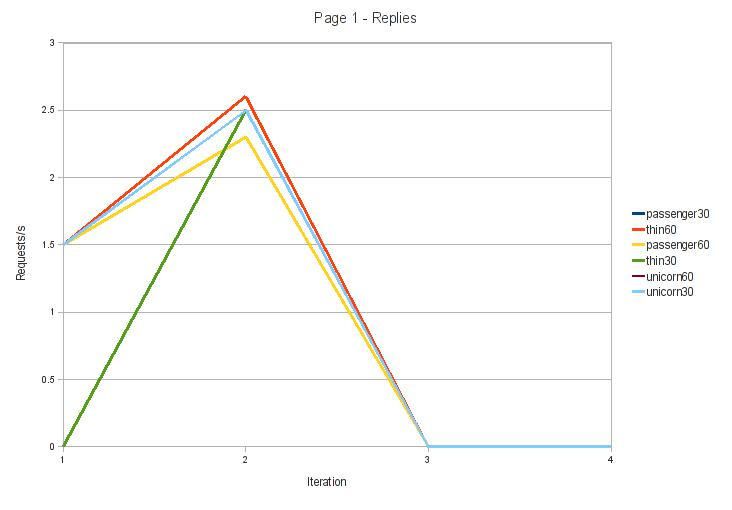
\includegraphics[width=0.95\textwidth]{results_autobench_replies_homepage_ruby18}
  \label{fig:page1_autobench_ruby18_results}
\end{figure}

The test tool, \textit{autobench}, was unable to find a stable request rate on this page. All web servers behaved similarly poor. 

As for the regular page with moderate usage of dynamic content---page 2---the results can be found on figure~\ref{fig:page2_autobench_ruby18_results}.
\begin{figure}[h!]
  \centering
    \caption{Autobench Results on Page 2 (Ruby 1.8)}
    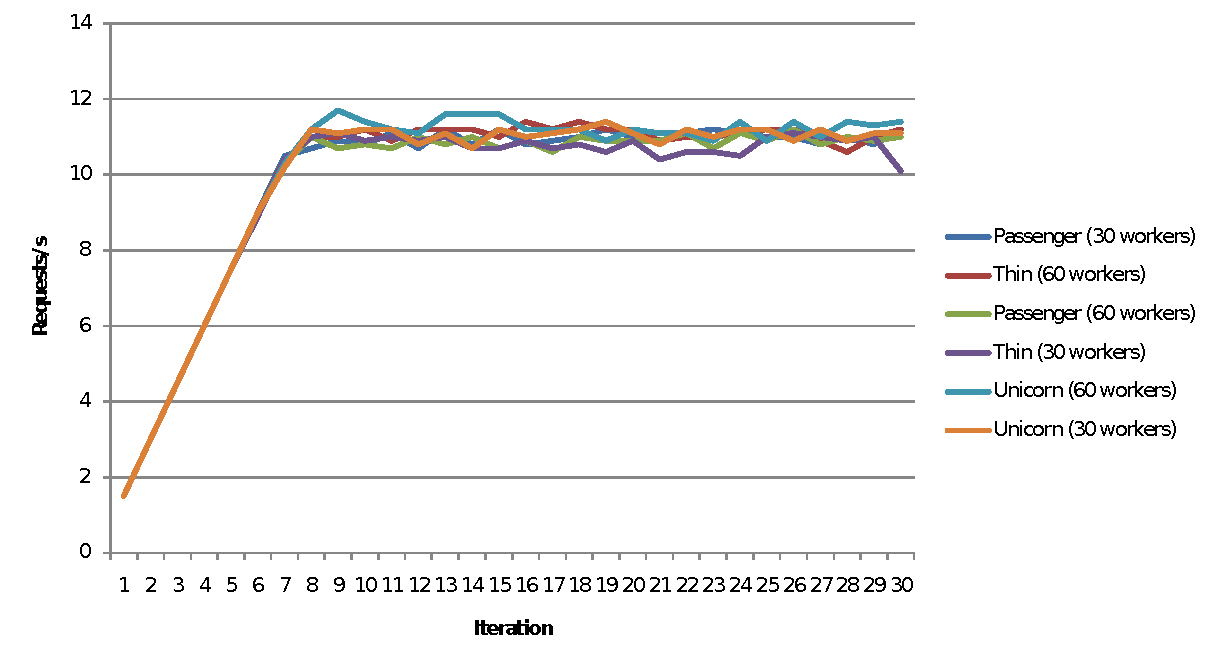
\includegraphics[width=0.95\textwidth]{results_autobench_replies_portal_ruby18}
  \label{fig:page2_autobench_ruby18_results}
\end{figure}

On this test all web servers were able to consistently serve requests, stabilizing at a rate of 10-12 requests per second. Although all had very similar performances, Unicorn with 60 workers consistently yielded slightly better results.

Finally, as for the complex but small API request---page 3---the results are exhibited on figure~\ref{fig:page3_autobench_ruby18_results}.
\begin{figure}[h!]
  \centering
    \caption{Autobench Results on Page 3 (Ruby 1.8)}
    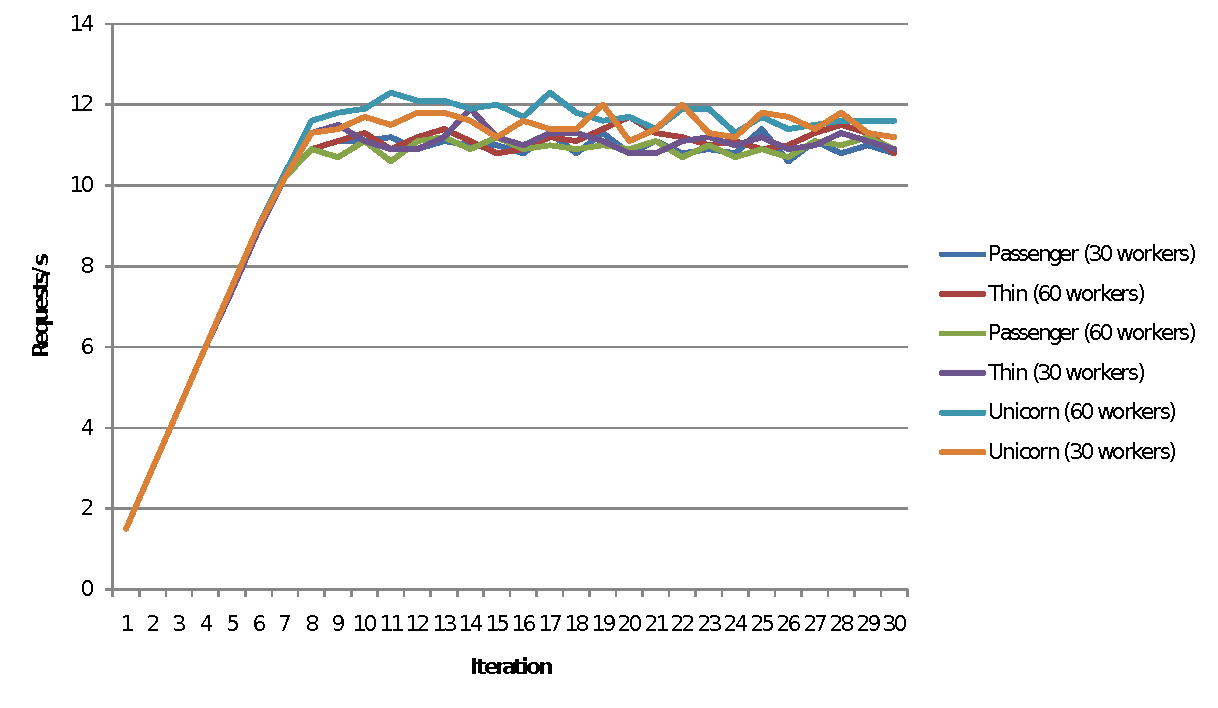
\includegraphics[width=0.95\textwidth]{results_autobench_replies_publication_ruby18}
  \label{fig:page3_autobench_ruby18_results}
\end{figure}

Once again, all web servers were able to maintain a solid request rate, which was stable around 10-13. Unicorn, both with 30 and 60 workers, seems to have a slight performance advantage over its competitors.

The second round was made using Ruby 1.9 on exactly the same pages. The results for the heavy page filled with dynamic content---page 1---can be seen on figure~\ref{fig:page1_autobench_ruby19_results}.
\begin{figure}[h!]
  \centering
    \caption{Autobench Results on Page 1 (Ruby 1.9)}
    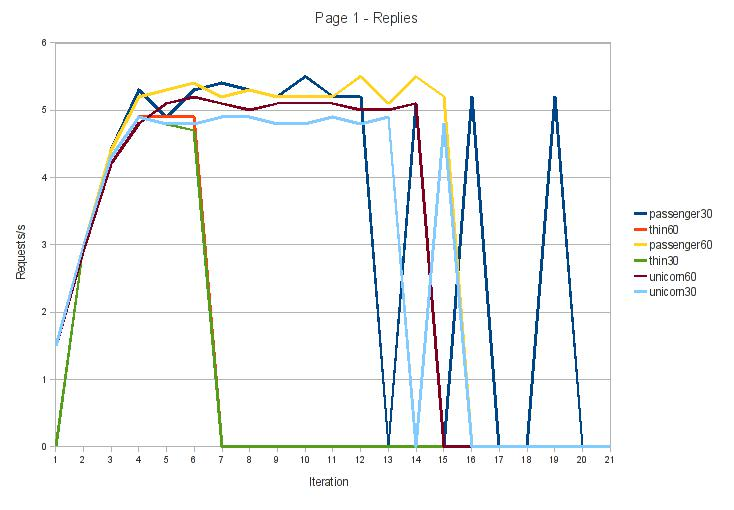
\includegraphics[width=0.95\textwidth]{results_autobench_replies_homepage_ruby19}
  \label{fig:page1_autobench_ruby19_results}
\end{figure}

All web servers have shown extreme improvements after switching to Ruby 1.9 on this page. Most of them were stable through 15-16 iterations instead of a single one and the response rate increased from 2,5 to 4,5-5,5. Thin is the most notable exception, loosing stability after 6 iterations. However, it still represents a remarkable improvement over the previous tests with Ruby 1.8.

As for the regular page with moderate usage of dynamic content---page 2---the results are presented on figure~\ref{fig:page2_autobench_ruby19_results}.
\begin{figure}[h!]
  \centering
    \caption{Autobench Results on Page 2 (Ruby 1.9)}
    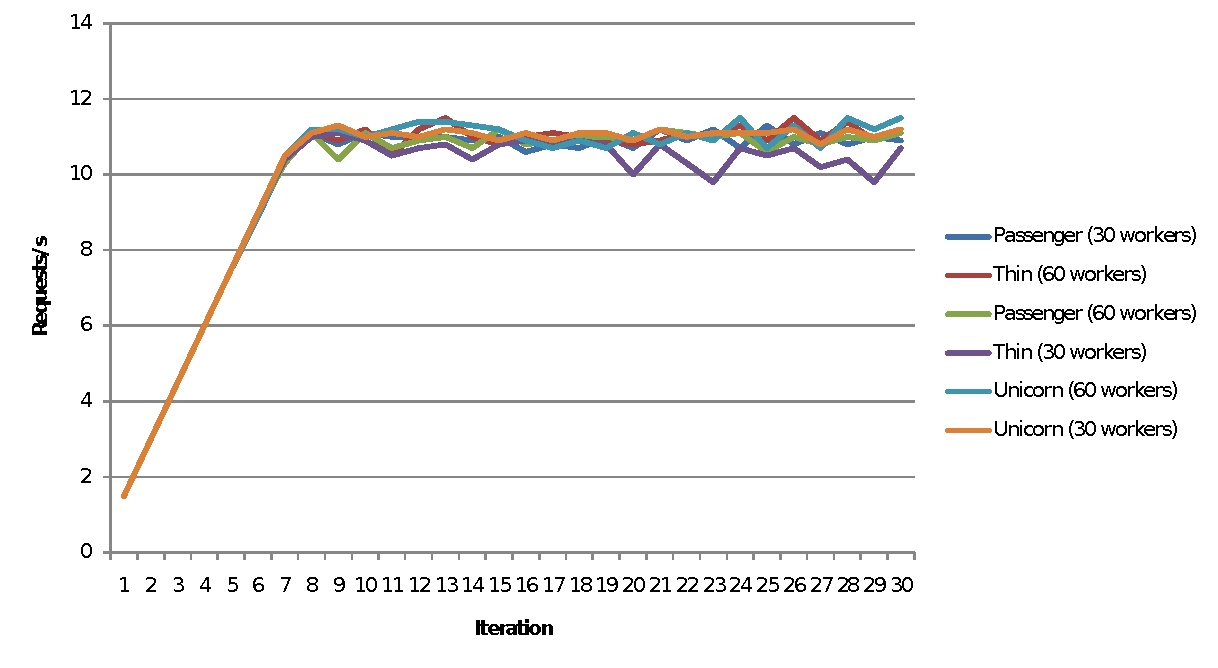
\includegraphics[width=0.95\textwidth]{results_autobench_replies_portal_ruby19}
  \label{fig:page2_autobench_ruby19_results}
\end{figure}

All web servers performed similarly on this test. The results were also very similar to the same test with Ruby 1.8, mainly due to the fact that this page is relatively light on Ruby code.

Finally, as for the complex but small API request---page 3---the results can be found on figure~\ref{fig:page3_autobench_ruby19_results}.
\begin{figure}[h!]
  \centering
    \caption{Autobench Results on Page 3 (Ruby 1.9)}
    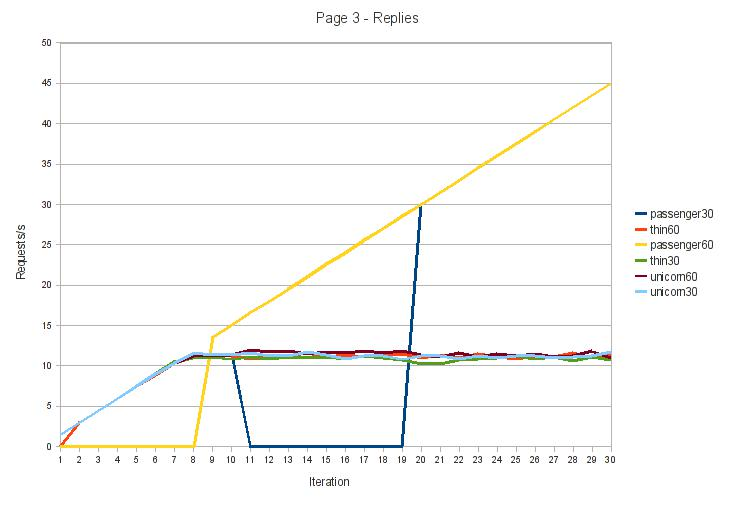
\includegraphics[width=0.95\textwidth]{results_autobench_replies_publication_ruby19}
  \label{fig:page3_autobench_ruby19_results}
\end{figure}

Once again, the results are very similar to those found on the same test with Ruby 1.8. Passenger's behavior is not consistent because its application handler segmentation faults on this specific test---complex API call on Ruby 1.9 with 30 and 60 workers---which is possibly related with shared resource access among workers.

Table~\ref{tab:web_server_memory_usage} exhibits the average memory usage throughout the test. A few conclusions can drawn from the memory usage data. Firstly, Thin always uses less memory than the other web servers. Passenger's memory usage with 30 workers is similar to when it is using 60 workers, which is very high when compared to the others. Finally, using Ruby 1.9 generally causes web servers to use less memory.
\begin{table}[h!t]
  \centering
  \caption{Web Server Memory Usage}
  \label{tab:web_server_memory_usage}
  
  \begin{tabular}{l|c|c|c|c|c|c}

     & \multicolumn{2}{c|}{\textbf{\textsc{Page 1}}} & \multicolumn{2}{c|}{\textbf{\textsc{Page 2}}} & \multicolumn{2}{c}{\textbf{\textsc{Page 3}}} \\ \hline
     & \textbf{Ruby 1.8} & \textbf{Ruby 1.9} & \textbf{Ruby 1.8} & \textbf{Ruby 1.9} & \textbf{Ruby 1.8} & \textbf{Ruby 1.9} \\ \hline
    \textbf{Thin (30)} & 3041 & 2868 & 3018 & 2802 & 2984 & 2849 \\ \hline
    \textbf{Unicorn (30)} & 3463 & 3556 & 3461 & 3354 & 3461 & 3442 \\ \hline
    \textbf{Passenger (30)} & 7794 & 6920 & 7661 & 6650 & 7666 & 6486 \\ \hline
    \textbf{Thin (60)} & 7214 & 6721 & 6993 & 6206 & 6995 & 6488 \\ \hline
    \textbf{Unicorn (60)} & 6808 & 6878 & 6804 & 6566 & 6803 & 6684 \\ \hline
    \textbf{Passenger (60)} & 7798 & 6921 & 7771 & 6687 & 7771 & 8045 \\
  \end{tabular}
\end{table}

After an exhaustive analysis of web servers performance, scalability and memory usage, one can conclude that the differences between web server performance are very small. The area of more impact is memory usage where Thin yields the best results, closely followed by Unicorn. Using Ruby 1.9, however, induces a significant improvement in the results regarding the response rate ability and the stability of all web servers. This difference is clearly noticeable in the heaviest test of the benchmark, where most web servers have shown a $\pm$200\% increase in the request rate and $\pm$1500\% increase in successfully completed iterations.

Most of the tests have shown small to no improvements when doubling the number of workers from 30 to 60. The main bottleneck is related to the nonexistence of a memory object caching system, so increasing the workers had no effect on performance. In fact, the difference between the results of this benchmark and the previously shown ones, with only 4 workers, is remarkably small. Database caching should be in use to precisely determine the difference between having 30 and 60 workers on the aforementioned dual-core machine.

\subsection{Tweaking}
Tweaking a web server's configuration is important to fine-tune its performance. All the examined components are highly configurable and changing some settings can provoke a positive or negative impact in performance.

Apache supports two completely different MPM models. A prefork MPM, which forks a number of identical Apache processes and a worker MPM, which creates multiple threads. The prefork model is generally more effective on systems with one or two processing units where the operating systems is better geared toward time slicing between multiple processes. When more CPUs are available, the worker model will probably be more effective. There are also important settings to address like, for instance, defining the maximum simultaneous connections that Apache can handle using \text{MaxClients} and setting the minimum and maximum number of spare threads/processes.

Unlike Apache, Nginx does not rely on threads nor processes to handle requests. Using a philosophy very similar to Thin's, it aims at solving the C10K problem~\footnote{\url{http://www.kegel.com/c10k.html}} by using an event-driven asynchronous architecture. Nginx supports various event models for handling connections which are optimized for certain situations or operating systems. The user must be certain that it is using the correct one for his system. One of the most efficient models---\textit{epool}---is only supported on Linux systems running a kernel in at least version 2.6, for instance.

Similarly to Apache's worker MPM, Cherokee is a threaded web server. However, it relies on the operating system for request queuing so it also supports many polling methods which are optimized for some systems, like \textit{epoll}. The amount of threads can and should also be configured specifically for each application and machine.

Thin itself is not as configurable as the previously mentioned web servers. However, there are important settings like, for instance, the maximum number of connections, that can be fine-tuned. As mentioned on section~\ref{tech:sec:rails_webservers}, Thin recently became capable of operating in a threaded manner by having a background pool of threads, despite its ``single process single thread'' philosophy. The following section will present a benchmark on this option.

Passenger has a significant amount of configuration options. One of the most important of them all is the process spawning method. While setting it to ``smart'' yields the best results according to its development team, it can cause incompatibilities with some \textit{gems}. The developers must test each system and see if this spawning method is suitable or not. Other interesting options include the number of requests interval in which an application process is restarted, useful for when an application has memory leaks.

Unicorn is a very configurable web server. Its configuration is written in Ruby and there is the possibility to hook into many parts of the start and execution processes. Among all options, there is one that is particularly interesting since it can change the size of the buffers which send and receive TCP data. These can be configured to match the kernel ones---defined by \textit{sysctl}---for optimal performance.

\subsubsection{Thin Performance with Threading Enabled}
Thin recently started to offer the an option which, when activated, will cause requests to be dispatched in a background pool of 20 threads. This slightly contradicts its initial ``single process single thread'' philosophy, though it still relies on an asynchronous event loop for each thread.

A benchmark comparing Thin's performance when threading is enabled or disabled was made using the three previously mentioned pages. Four workers were used in each test and, like the initial benchmarks, \textit{ab} as used to conduct each test. The results are exhibited on table~\ref{tab:thin_threaded_benchmark}.

\begin{table}[h!t]
  \centering
  \caption{Thin with Threading Benchmark Results}
  \label{tab:thin_threaded_benchmark}
  
  \begin{tabular}{c|c|c|c|c|c}

    \textbf{Req. / Conc.} & \textbf{Page} & \textbf{Web Server} & \textbf{Requests/s (\#)} & \textbf{Total time (s)} & \textbf{Mem. Usage (B)} \\ \hline
    \multirow{6}{*}{50/1} & \multirow{2}{*}{API} & Thin & \textbf{9.24} & \textbf{5.411} & \textbf{121213}\\\cline{3-6}
     &  & Thin(threaded) & 7.5 & 6.665 & 126491\\\cline{2-6}
     & \multirow{2}{*}{Heavy} & Thin & \textbf{1.22} & \textbf{41} & \textbf{121506}\\\cline{3-6}
     &  & Thin(threaded) & 0.91 & 55.221 & 128809\\\cline{2-6}
     & \multirow{2}{*}{Regular} & Thin & \textbf{5.99} & \textbf{8.341} & \textbf{121325}\\\cline{3-6}
     &  & Thin(threaded) & 4.67 & 10.711 & 126954\\\hline
    \multirow{6}{*}{100/10} & \multirow{2}{*}{API} & Thin & \textbf{11.84} & \textbf{8.444} & \textbf{121412}\\\cline{3-6}
     &  & Thin(threaded) & 11.81 & 8.465 & 128097\\\cline{2-6}
     & \multirow{2}{*}{Heavy} & Thin & \textbf{2.25} & \textbf{44.495} & \textbf{121666}\\\cline{3-6}
     &  & Thin(threaded) & 1.84 & 54.468 & 133241\\\cline{2-6}
     & \multirow{2}{*}{Regular} & Thin & \textbf{12.14} & \textbf{8.236} & \textbf{121402}\\\cline{3-6}
     &  & Thin(threaded) & 11.73 & 8.527 & 128709\\\hline
    \multirow{6}{*}{500/50} & \multirow{2}{*}{API} & Thin & \textbf{11.67} & \textbf{42.332} & \textbf{121593}\\\cline{3-6}
     &  & Thin(threaded) & 11.47 & 43.605 & 129938\\\cline{2-6}
     & \multirow{2}{*}{Heavy} & Thin & \textbf{2.37} & \textbf{212.427} & \textbf{125128}\\\cline{3-6}
     &  & Thin(threaded) & FAIL & FAIL & 152066\\\cline{2-6}
     & \multirow{2}{*}{Regular} & Thin & \textbf{12.45} & \textbf{40.173} & \textbf{121625}\\\cline{3-6}
     &  & Thin(threaded) & 11.9 & 42.005 & 130860\\\hline
    \multirow{6}{*}{500/100} & \multirow{2}{*}{API} & Thin & 11.48 & 43.546 & \textbf{121613}\\\cline{3-6}
     &  & Thin(threaded) & \textbf{11.6} & \textbf{43.111} & 130082\\\cline{2-6}
     & \multirow{2}{*}{Heavy} & Thin & \textbf{2.45} & \textbf{203.037} & \textbf{127759}\\\cline{3-6}
     &  & Thin(threaded) & FAIL & FAIL & 139153\\\cline{2-6}
     & \multirow{2}{*}{Regular} & Thin & \textbf{12.54} & \textbf{39.883} & \textbf{121650}\\\cline{3-6}
     &  & Thin(threaded) & 11.68 & 42.818 & 130909\\\hline
    \multirow{6}{*}{2500/500} & \multirow{2}{*}{API} & Thin & FAIL & FAIL & \textbf{122012}\\\cline{3-6}
     &  & Thin(threaded) & FAIL & FAIL & 130558\\\cline{2-6}
     & \multirow{2}{*}{Heavy} & Thin & FAIL & FAIL & \textbf{127524}\\\cline{3-6}
     &  & Thin(threaded) & FAIL & FAIL & 134980\\\cline{2-6}
     & \multirow{2}{*}{Regular} & Thin & FAIL & FAIL & \textbf{122020}\\\cline{3-6}
     &  & Thin(threaded) & FAIL & FAIL & 131290\\
  \end{tabular}
\end{table}

Threaded Thin actually performs worse in these test pages. It uses slightly more memory and generally needs a small amount of extra time to complete each test. Threads have an associated overhead, mainly related to the spawning process and the context switches they provoke. Since Thin is based on a really fast asynchronous loop, it is likely that this processing overhead is, in this case, slowing the web server down overall.

\section{Databases} % (fold)
\label{solution:sec:databases}

Concerning databases, the emerging MySQL Ruby library---\textit{mysql2}---was targeted for improvements.

A database, from Rails' perspective, is all about choice. There are three different natively supported relational databases including SQLite, MySQL and PostreSQL. The community, however, as given third-party support to many alternative relational and non-relational databases including MongoDB, CouchDB, DataMapper, SQL Server and Oracle, to name a few.

The popularity of non-relational databases is increasing among the Rails' community, trading enhanced read and write speeds for higher disk usages and fewer functionalities. However, as mentioned on Section~\ref{tech:sec:databases} most Rails applications rely on relational databases, mainly MySQL. On the other hand, benchmarking PostgreSQL against MySQL was discarded as a worthy task because of what was already exposed in Section~\ref{state:sec:databases}. Finally, adapting \textit{Escolinhas.pt} to a non-relational database for further evaluation would require a significant amount of refactoring and some deep architectural changes, being discarded as a possible approach to this component. For these reasons, MySQL was the chosen database to address in this thesis's context.

Due to the aforementioned Rails-centric perspective and the higher probability of success in the medium term, it was not the database itself that was targeted for improvements but instead a recent, improved Ruby database library---\textit{mysql2}. As mentioned in Section~\ref{state:sec:databases}, this Ruby MySQL library can yield results up to 400\% better than the default library in an optimal situation. However, there are caveats which need to be addressed, as explored in the following section.

Improving \textit{mysql2} was the general goal of the work presented in this section.

\subsection{Development}
As mentioned in Chapter~\ref{cha:problem_statement}, \textit{mysql2} handles the conversion of the data between MySQL types and Ruby objects immediately after fetching each row from the database. Since the conversion itself is done in C, there are significant performance improvements over the current default MySQL library which returns all results as ``strings'', forcing Rails to make the conversions in Ruby. 

There are, however, caveats to the approach used by \textit{mysql2}. Since the type conversion is not lazy casted, there is a possibility that the library is converting unnecessary data. If the developer fetches a significant amount of rows from the database but then only uses a small portion of those rows, the library is likely to have a similar or worse performance than the default library. This happens because unlike \textit{mysql2}, using the default database driver Rails will lazy type cast the ``strings'' it receives, only converting the really necessary data.

Adding lazy type casting to fields in \textit{mysql2} was developed in conjunction with one of the library's core developer, Brian Lopez. The changes are still under the core team's development process. There are many optimizations currently being made and support for some uncommon MySQL data types is still being developed and added. For this reason, the changes are not present in the current public release of this database library and there are also no reliable benchmarks to determine the real improvements over the old version of \textit{mysql2} or other MySQL adapters. However, a patch with the changes which can be applied to the library's source code\footnote{\url{http://github.com/brianmario/mysql2/}} is presented on appendix~\ref{ap:mysql2_patch}.


\subsection{Section Overview}
This section exhibited and explained the work concerning databases. A promising Ruby library for MySQL was improved, by changing its behavior concerning database field casting. Instead of converting all fields from MySQL types to Ruby objects upon fetching, it now lazy type casts them as needed.

Adding lazy type casting to \textit{mysql2} allowed to fulfill the general goal initially stated---this library's worst performing case has been reduced by solving one of its biggest caveats.

\section{Ruby on Rails} % (fold)
\label{solution:sec:ruby_on_rails}
The main focus related with Ruby on Rails itself was to improve the current tools for profiling and benchmarking applications. Motivating the adoption of the soon to be released version of this framework---Rails 3---by the community was also a goal regarding this component. Increasing the community's awareness of this subject was also addressed by publishing an article to a popular magazine and engaging in a summer project---Ruby Summer of Code---with high visibility. Nonetheless, some common pitfalls were also addressed while presenting and benchmarking their solutions.

Improving Rails' profiling tools, motivating the adoption of Rails 3 and increasing the community's awareness of this subject were the general goals of the work presented in this section.


\subsection{Benchmarking}
Rails developers can often incur in some development performance pitfalls which can easily be addressed by using some of Rails' powerful functionalities. This section will cover some of these possible pitfalls, propose solutions and generally assert their performance differences.


\subsubsection{Eager Loading}
Eager loading is a core feature of Ruby on Rails which, in certain situations, can lead to significant performance slowdowns because of its absence or misuse. It allows the developer to specify if and which associations should be loaded up front, being the opposite of lazy loading. A classical example of the usefulness of this feature consists in a blog post with comments in which rendering the post's page will also render its comments. Eager loading allows the developer to specify that the comments should be loaded alongside the post, instructing Rails to only use two database queries---one for the post and another for its comments. If not explicitly specified, Rails will load each comment independently while rendering them. Loading the post and eager loading its comments is illustrated in the following code.
\begin{lstlisting}[xleftmargin=30pt,xrightmargin=30pt]
@posts = Post.find(:all, :include => :comments)
\end{lstlisting}

A simple benchmark was performed on a scaffold blog Rails application. The Rails version in use was 2.3.5. The database in use was MySQL using Ruby's default library. A thousand blog posts were generated automatically, along with two hundred thousand comments randomly associated with blog posts. This benchmark compares the time needed to complete a request which fetches all posts along with their comments. The test was run five times to eliminate circumstantial issues and the best results are shown. The results are exhibited on table~\ref{tab:eager_loading}.
\begin{table}[h!t]
  \centering
  \caption{Eager Loading Benchmark Results}
  \label{tab:eager_loading}
  
  \begin{tabular}{c|c}
  
    \textbf{\textsc{Eager Loading}} & \textbf{\textsc{Time (seconds)}} \\
    \hline
    No & 283 \\ \hline
    Yes & 21 \\
  \end{tabular}
\end{table}

In this extreme example, eager loading the data took $\pm$7\% of the time needed to lazy load the data, which is Rails default behavior. Eager loading can have a significant performance impact, depending on the context, as exemplified.


\subsubsection{Transactions}
Rails wraps every database write and update inside a transaction if not instructed otherwise. This happens because of its before/after filter functionality, which allows developers to hook code before and after certain actions are executed. In these cases, the operation and its filters are wrapped inside a transaction.

There are cases, however, where this behavior is suboptimal. When write/update calls are being executed consecutively---for instance, inside a loop---all database calls will be inside their own transaction. This will incur in significant performance penalties, depending on the amount of database actions. However, Rails allows developers to specify where the transaction should begin and end. The following code exemplifies this statement.
\begin{lstlisting}[xleftmargin=30pt,xrightmargin=30pt]
ActiveRecord::Base.transaction do
  (1..100).each { |i| Number.create(:value => i) }
end
\end{lstlisting}
In this example, instead of using one hundred transactions Rails will only use a single one. Using the same environment from the benchmark in the previous section, a benchmark was conducted on asserting the performance difference in explicitly using a global transaction instead of letting Rails place many small transactions which is, as previously mentioned, its behavior by default. This benchmark consisted in creating posts and associated comments, all with the same content. Two tests were made, the first by creating one hundred posts with twenty comments each and a second one by creating one post with two comments. Results can be seen on table~\ref{tab:transaction}.
\begin{table}[h!t]
  \centering
  \caption{Explicit Transaction Benchmark Results}
  \label{tab:transaction}
  
  \begin{tabular}{c|c|c}
  
    & \textbf{\textsc{Explicit Transaction}} & \textbf{\textsc{Time (milliseconds)}} \\ \hline
    100 posts, 20 comments & No & 76017 \\ \hline
    100 posts, 20 comments & Yes & 5223 \\ \hline
    1 post, 2 comments & No & 176 \\ \hline
    1 post, 2 comments & Yes & 137 \\
  \end{tabular}
\end{table}

Using a global transaction on the heaviest test implied a $\pm$93\% reduction on the time needed to write the data. On the lighter test, however, this reduction was of $\pm$22\%. On consecutive writes and/or updates, using a global transaction can significantly increase the performance of the operation.


\subsubsection{Magic Finders}
Rails has a feature commonly called ``magic finders''. It improves code's readability by allowing the developer to replace some calls with smaller and more readable ones. The following example illustrates this feature, comparing with a regular call.\\\\\\ % FIXME: next page?
\begin{lstlisting}[xleftmargin=30pt,xrightmargin=30pt]
Comment.find(:first, :conditions => ["created_at = ?", "2009-11-06 18:25:48"]) # normal find

Comment.find_by_created_at("2009-11-06 18:25:48") # magic find
\end{lstlisting}
These calls, however, have an associated performance penalty. Using the same test environment found on the previous benchmarks, both previously presented calls were benchmarked. The results are presented on table~\ref{tab:magic_finders}.
\begin{table}[h!t]
  \centering
  \caption{Magic Finders Benchmark Results}
  \label{tab:magic_finders}
  
  \begin{tabular}{c|c}
  
    \textbf{\textsc{Type}} & \textbf{\textsc{Time (milliseconds)}} \\ \hline
    Normal find & 62 \\ \hline
    Magic find & 197 \\
  \end{tabular}
\end{table}

The normal find only takes $\pm$32\% of the time needed by the magic find to complete. Since there is a readability/performance trade-off, using either syntaxes is a decision which depends on the project and its developers. The general performance penalty associated with the commonly used magic finders is, however, significant and should be taken into account.


\subsubsection{Fetching Large Groups of Records}
In certain situations, Rails applications need to fetch a significant amount of rows from the database, instantiate each model object and render them in a view. Using the ``find'' helper, this operation can be significantly heavy on memory, as it fetches and loads all records into Ruby objects, and will lock the application until all operations are complete.

However, when Rails 2.3 was introduced it bundled a couple of methods which are likely to be very useful in these situations: ``find\_each'' and ``find\_in\_batches''. The first will retrieve a specified amount of objects at a time, letting the code iterate over the records as if it was a normal ``find'' call. The second is very similar, except that it gives control back to the application every time it fetches a batch. Both methods have a ``batch\_size'' option which defaults to one thousand records. These additional methods have the advantage of using less memory and, as explored in Section~\ref{state:sec:ruby}, less memory usage will trigger Ruby's garbage collector less often, providing better execution times. Notwithstanding these advantages, these methods are unlikely to yield performance improvements when fetching small amounts of records.

To accurately determine the performance benefits involved with switching the ``find'' call with ``find\_each'' when there is a significant amount of records involved, a benchmark was done. The environment was the same as previous benchmarks. The test itself consisted in fetching the two hundred thousand comments in the example blog application. The results can be found on table~\ref{tab:fetch_in_batches}.
\begin{table}[h!t]
  \centering
  \caption{Fetching Records in Batches Benchmark Results}
  \label{tab:fetch_in_batches}
  
  \begin{tabular}{c|c|c}
  
    \textbf{\textsc{Method}} & \textbf{\textsc{Time (seconds)}} & \textbf{\textsc{Memory Usage (MB)}} \\ \hline
    find & 211 & 158 \\ \hline
    find\_each & 195 & 118 \\
  \end{tabular}
\end{table}

Using the alternative method to fetch records in batches, the application needed 10\% less time to fetch the records and used 25\% less memory. These are significant improvements, mainly in memory usage.

\subsection{Development}
The development phase regarding this component involved many distinct activities. First of all, it was crucial to refactor Rails' native profiling and benchmarking tools. Taking into consideration that the release of the new version of the Ruby on Rails framework is nearing, it was important to motivate its early adoption by porting some widely used plugins/gems and one of this framework's most famous applications to the most recent version. After that, a small task related to adding support for the Nginx's \textit{X-Accel-Redirect} header to Rails was performed. Finally, an overview on the current work under the Ruby Summer of Code program is given.


\subsubsection{Refactoring Rails Profiling/Benchmarking Tools}
Rails' profiling and benchmarking tools were nonfunctional on YARV, as they relied on Rub 1.8's now outdated architecture. Ruby evolved very fast and these tools did not keep up, becoming deprecated and useless when used on this version.

Adding Ruby 1.9  support to these tools was crucial, since developers could not rely on the native tools when benchmarking and profiling their applications. By taking advantage of the enhances made to Ruby's profiling tools mentioned in Section~\ref{solution:sec:ruby}, Rails was overhauled~\footnote{\url{http://github.com/rails/rails/commits/master?author=goncalossilva}} and now fully supports profiling and benchmarking under Ruby 1.9.


\subsubsection{Porting Plugins to Rails 3}
Rails 3 adoption by developers is highly conditioned by plugin availability. As mentioned in Section~\ref{tech:sec:ruby_on_rails}, there is a significant amount of plugins available for Ruby on Rails. However, due to the recent Rails' architectural changes, authors generally need to update their plugins/gems to be compatible to this version. The lack of available plugins will certainly limit the adoption rate of this version. In order to help alleviating this problem, some famous plugins were updated to comply with the new Rails API for plugins/gems. All plugins used by \textit{Escolinhas.pt} were analyzed and the ones with the higher watcher count\footnote{GitHub allows users to start ``watching'' repositories, being notified of all changes made to the projects they ``watch''} on their public repositories, were selected. Their names and functionality are:
\begin{description}
  \item[acts\_as\_list,] a plugin for sorting and reordering a number of objects in a list\footnote{\url{http://github.com/goncalossilva/acts_as_list/}};
  \item[permalink\_fu,] a plugin for creating URL-friendly permanent links from object attributes\footnote{\url{http://github.com/goncalossilva/permalink_fu/}};
  \item[acts\_as\_paranoid,] a plugin for hiding records instead of deleting them, being able to recover them\footnote{\url{http://github.com/goncalossilva/rails3_acts_as_paranoid/}}.
\end{description}
All the mentioned plugins were refactored to use the new plugin API. Some tests also needed refactoring, as they used deprecated Rails code. However, updating \textit{permalink\_fu} also involved replacing its character conversion engine since it relied on deprecated Ruby 1.8 functionality, meaning this plugin was not compatible with Ruby's most recent version. On the other hand, \textit{acts\_as\_paranoid} had to be completely rewritten. It was initially developed for Rails 1 and slightly patched to work on Rails 2, having a deprecated architecture which was incompatible with Rails 3. Recreating this plugin from ground up with Rails 3 in mind allowed a $\pm$70\% reduction in lines of code.


\subsubsection{Porting Redmine to Rails 3}
Redmine\footnote{\url{http://www.redmine.org/}} is an open-source flexible project management web application written in Ruby on Rails, created by Jean-Philippe Lang. It is one of the most famous open-source Rails projects, having more than 90 reported major installations worldwide~\cite{redmine_installations}, including the development teams of Ruby, phpBB and Lighttpd. It is a complex platform with over 60 models and 65000 lines of code.

Redmine was upgraded to be compatible with Rails 3 and the source code is hosted at GitHub\footnote{\url{http://github.com/goncalossilva/redmine}}. This upgrade increased Rails 3's visibility while showing the potential performance improvements in upgrading, since this version is reportedly faster. The benefits can be experienced by the users themselves while using Redmine. Many issues had to be addressed, including fixes on the application initialization process, string handling, parameter filtering, plugin support, usage of Javascript helpers and method overriding, among others. All changes can be explored in detail on the project's commit log at GitHub.


\subsubsection{Adding X-Accel-Redirect Support to Rails}
Rails lacks support for Nginx's \textit{X-Accel-Redirect} header by default, so a plugin to add it was developed\footnote{\url{http://github.com/goncalossilva/X-Accel-Redirect}}. Similar to Apache's \textit{X-Sendfile}, \textit{X-Accel-Redirect} can be useful when a user requests the download of a file from the server. If this flag is set on the response body, it will instruct Nginx to handle the file delivery itself. This way, the Rails process will be free to handle other requests instead of blocking to serve the file, delegating that task to Nginx.


\subsubsection{Benchmarking Continuous Integration}
Late in this project's course, applications for the Ruby Summer of Code\footnote{\url{http://www.rubysoc.org/}} began. This program is similar to Google Summer of Code, being a student internship program designed to help fund student development of Ruby-related projects during the summer.

The decision to apply for this program was made, by proposing the development of a Benchmarking Continuous Integration for Ruby on Rails. This proposal was later accepted and a project mentor assigned---Yehuda Katz. Yehuda, the lead developer of the discontinued Merb framework, is one of the most prominent developers behind Rails 3, having joined the core team as soon as the decision to merge Rails and Merb became official.

``Project \#8: Benchmarking CI\footnote{\url{http://www.rubysoc.org/projects/}}'' consists in building an official full-stack benchmarking suite for Ruby on Rails. This way, each commit to the Rails repository will automatically trigger a process where a remote machine starts a new server, runs the tests and reports back the results. As time goes by, it will be possible to watch the evolution of the framework's performance and developers will be able to keep track of the impact their changes have. Any performance regressions will be detected and the responsible developers notified. In its most basic form, it will bring a kind of performance-oriented continuous integration for the Ruby on Rails framework.

The whole Rails community will benefit from having an official benchmarking suite for Ruby on Rails. On one hand, developers will have increased awareness of the framework's performance. They will be able to benchmark their changes and understand their impact on every component, making small adjustments if any significant performance regressions are found. On the other hand, the community will also benefit since Rails will definitely become faster and more scalable over time.


\subsection{Community Blog}
Soon after the start of the project, a public blog named ``Snap Rails''\footnote{\url{http://snaprails.tumblr.com}} was created. Many of the findings done throughout this project have been presented there. Despite being fairly recent, it already surpasses a thousand unique visitors. A map overlay showing their locations is shown on figure~\ref{fig:snaprails_map_overlay}.
\begin{figure}[h!t]
  \centering
    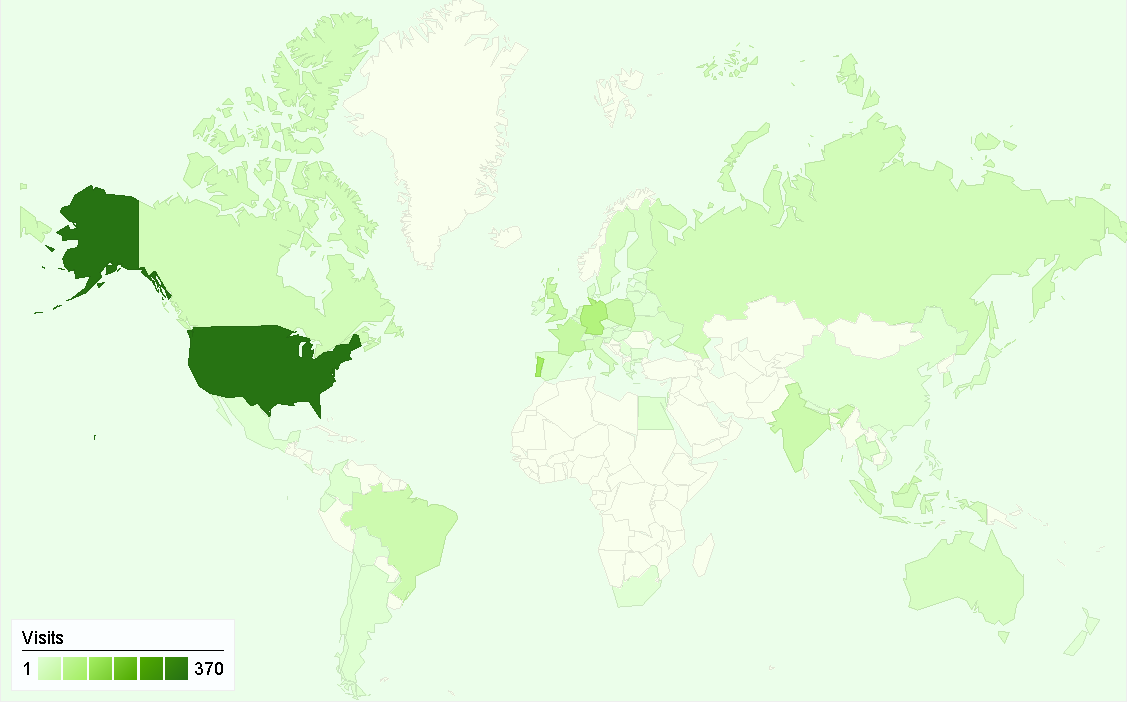
\includegraphics[width=0.75\textwidth]{snaprails_map_overlay}
    \caption{``Snap Rails'' Map Overlay} \label{fig:snaprails_map_overlay}
\end{figure}
Visitor analysis was made using Google Analytics\footnote{\url{http://analytics.google.com}}. With visitors from more than fifty five countries, this blog's purpose is to continuously increase this subject's visibility.


\subsection{Performance-oriented Article Series}
A series of performance-oriented articles for the \textit{Rails Magazine} has also begun. The first article is already present on the sixth edition of the magazine~\cite{rails_magazine_6}, with more to follow on future releases. Similarly to this thesis, this article performance series will cover all system's components, having already started with an introduction to this subject. A copy is exhibited in appendix~\ref{ap:rails_magazine}.

Publishing articles on this matter on such a popular magazine increases this subjects' visibility and the importance in building highly scalable Ruby on Rails applications, possibly igniting the community's awareness of this subject.


\subsection{Section Overview}
This section exhibited and explained the work concerning Ruby on Rails. Regarding benchmarking, common performance pitfalls and their solutions were analyzed. Concerning development, Rails' profiling and benchmarking tools were revamped and now seamlessly integrate with Ruby's. After that, some renowned plugins and Redmine were ported to Rails 3. A plugin which adds support for Nginx's \textit{X-Accel-Redirect} was also created. Finally, a project related to the creation of a performance-oriented continuous integration for Rails under the Ruby Summer of Code program was detailed. This section also presents some work that does not fit under the usual fields---benchmarking, development and tweaking---which is related with increasing the community's awareness of the importance of building highly performant Rails applications. This work is related with the creation of a community blog on this subject and the start of a performance-oriented series of articles for \textit{Rails Magazine}.

Making Rails' profiling tools agnostic to which Ruby version is using them and consequently seamless integrate with YARV allowed to improve these tools. Porting Redmine and various plugins to Rails 3 increased this version's visibility and eased the process of upgrading, motivating its adoption. Creating the general guidelines by using information from this and previous sections, starting a community blog and writing an article series are likely to increase the community's awareness of this subject. Finally, building a benchmarking continuous integration for Rails itself will also increase its developer's awareness of this subject, completing the last of the general goals initially stated.


